\cleardoublepage

\chapter[Computing the ED and SVD]{Computing the eigendecomposition and the singular value decomposition}

\label{chapter:algorithms}

We have looked at what PCA is, at how to understand it, and we have spent a full chapter on developing the tools necessary to prove the spectral theorem, the particular decomposition that makes it all possible.

What we haven't discussed yet, in any detail, is how to \emph{build it}. And how to build it efficiently. We've looked at the singular value decomposition (SVD) in great detail, and with an algorithm for computing the SVD available, computing the PCA is trivial. But that's kicking the can down the road. How then, do we implement the SVD?

In practice, you'll rarely have to build much of PCA from scratch, and if you do, there are better resources than this one to tell you what to pay attention to. 

\begin{aside}For instance, \emph{Matrix Computations} by \citet{golub2013matrix}.
\end{aside}

So why do we care about building a PCA implementation from scratch ourselves? Because building something is one of the best ways of understanding it. There are many things we don't yet understand, or understand well, about PCA, eigenvectors and singular vectors. By looking at some of the different ways you might implement PCA, we can learn a lot more about what it actually does.

So that will be our aim. We won't focus on the most popular algorithms, and we won't bother with all the tricks required to make the algorithms faster or more robust. We will simply set ourselves the challenge to implement PCA from scratch in a relatively efficient manner, but we will focus on those algorithms that illustrate most clearly what is happening when PCA is computed.

Remember that we've seen one algorithm already in Chapter~\ref{chapter:introduction}. There, we searched, using projected gradient descent, for the unit vector that gave us the best  reconstruction of the data from a single number. This gave us the first principal component, and from that we could search for the second one, and so on.

\begin{aside}We also briefly mentioned a version of this algorithm for the singular value decomposition in Chapter~\ref{chapter:svd}.
\end{aside}

Our job in this chapter is to do a little better. We'll still require iterative algorithms with approximate solutions, but we'll try to get away from approximating the principal components one by one. Finally, we'll do our best to show that our algorithms are guaranteed to converge, and if possible, give an idea of how fast they converge.

\section{Computing eigenvectors}

Our starting point will be the fact that we derived in Chapter~\ref{chapter:eigenvectors}: the principal components are the eigenvalues of the sample covariance matrix \(\bc{\mbS}\) of our data. All we need to do is to compute \(\bc{\mbS}\), and then figure out what its eigenvectors are. Along the way, we'll try to develop a little more insight into what eigenvectors are, and what they tell us about a matrix.

We'll look at three algorithms for computing eigenvectors that each build on one another: \textbf{power iteration}, \textbf{orthogonal iteration} and \textbf{QR iteration}.

\index{Power iteration}\index{Orthogonal iteration}\index{QR iteration}

Then, we'll switch to the alternative perspective we developed in Chapter~\ref{chapter:svd}: that the principal components are the \emph{singular vectors} of the \emph{data} matrix \(\mbX\), and we'll build on our three algorithms for computing eigenvalues to develop three algorithms along the same lines for computing the SVD.

\subsection[Power iteration: computing 1 eigenvector]{Power iteration: computing one eigenvector}

\index{Computing eigenvectors!by power iteration}
\index{Pagerank|(}

Before we get to the business of computing eigenvectors, allow me a little diversion. It will help us to build some more intuition for what eigenvectors are, and this intuition will become the foundation for all the algorithms that follow.

As ancient as it may make the rest of us feel, some people reading this will have become internet users only after Google was invented. If this is you, you will have no memory of how useless search engines were before Google came along. You won't have experienced the watershed that the introduction of Google was. You may not even believe that their almost-complete market dominance can be traced back to one simple idea.

The modern Google engine combines a vast array of methods and philosophies, but the original idea that set it so far apart from the competitors was singular, and simple.

Back then, the main problem facing search engines was the number of webpages trying to game the system. Authors would include fake keywords, large swathes of invisible text, everything they could think of to get as high in the results for as many different search terms as possible. This would inevitably lead to useless, nonsense-filled websites cluttering up search results.

What Google wanted to do was to develop a measurement of \emph{reputation}: a single number that could capture to what extent a website was a respectable source of information playing by the rules, versus a cheap ad-laden swindle, trying to attract clicks. Their basic idea was a \emph{social} one: if somebody, somewhere on the web chooses to link to you, they must trust you, and this should serve as a signifier of your reputation. The more people link to you the better your reputation.

\index{Reputation}

By itself, this notion of reputation is easy enough to game. Just set up a load of websites that all link to each other. But the idea can be applied \emph{recursively}: the better the reputation of the sites that link to you, the more they add to your reputation. And \emph{their} reputation is in turn determined by the reputation of the sites that link to \emph{them} and so on.

Theoretically, we could keep going forever, always avoiding the question of how we define the reputation of a website, by simply deferring the question to the reputation of the websites that link to it. In practice, we'll need to stop somewhere, and define the base reputation, independent of who links to it. It turns out however, that if we defer the question for a large number of steps, it doesn't much matter what we do when the recursion stops. We can simply assign all websites we find at that point a reputation of 1, and the main thing that will determine the reputation of the site we started with will be the structure of the graph of links, not the constant reputation we assigned to the websites at which we stopped.

\begin{figure}[H]
	\centerline{
		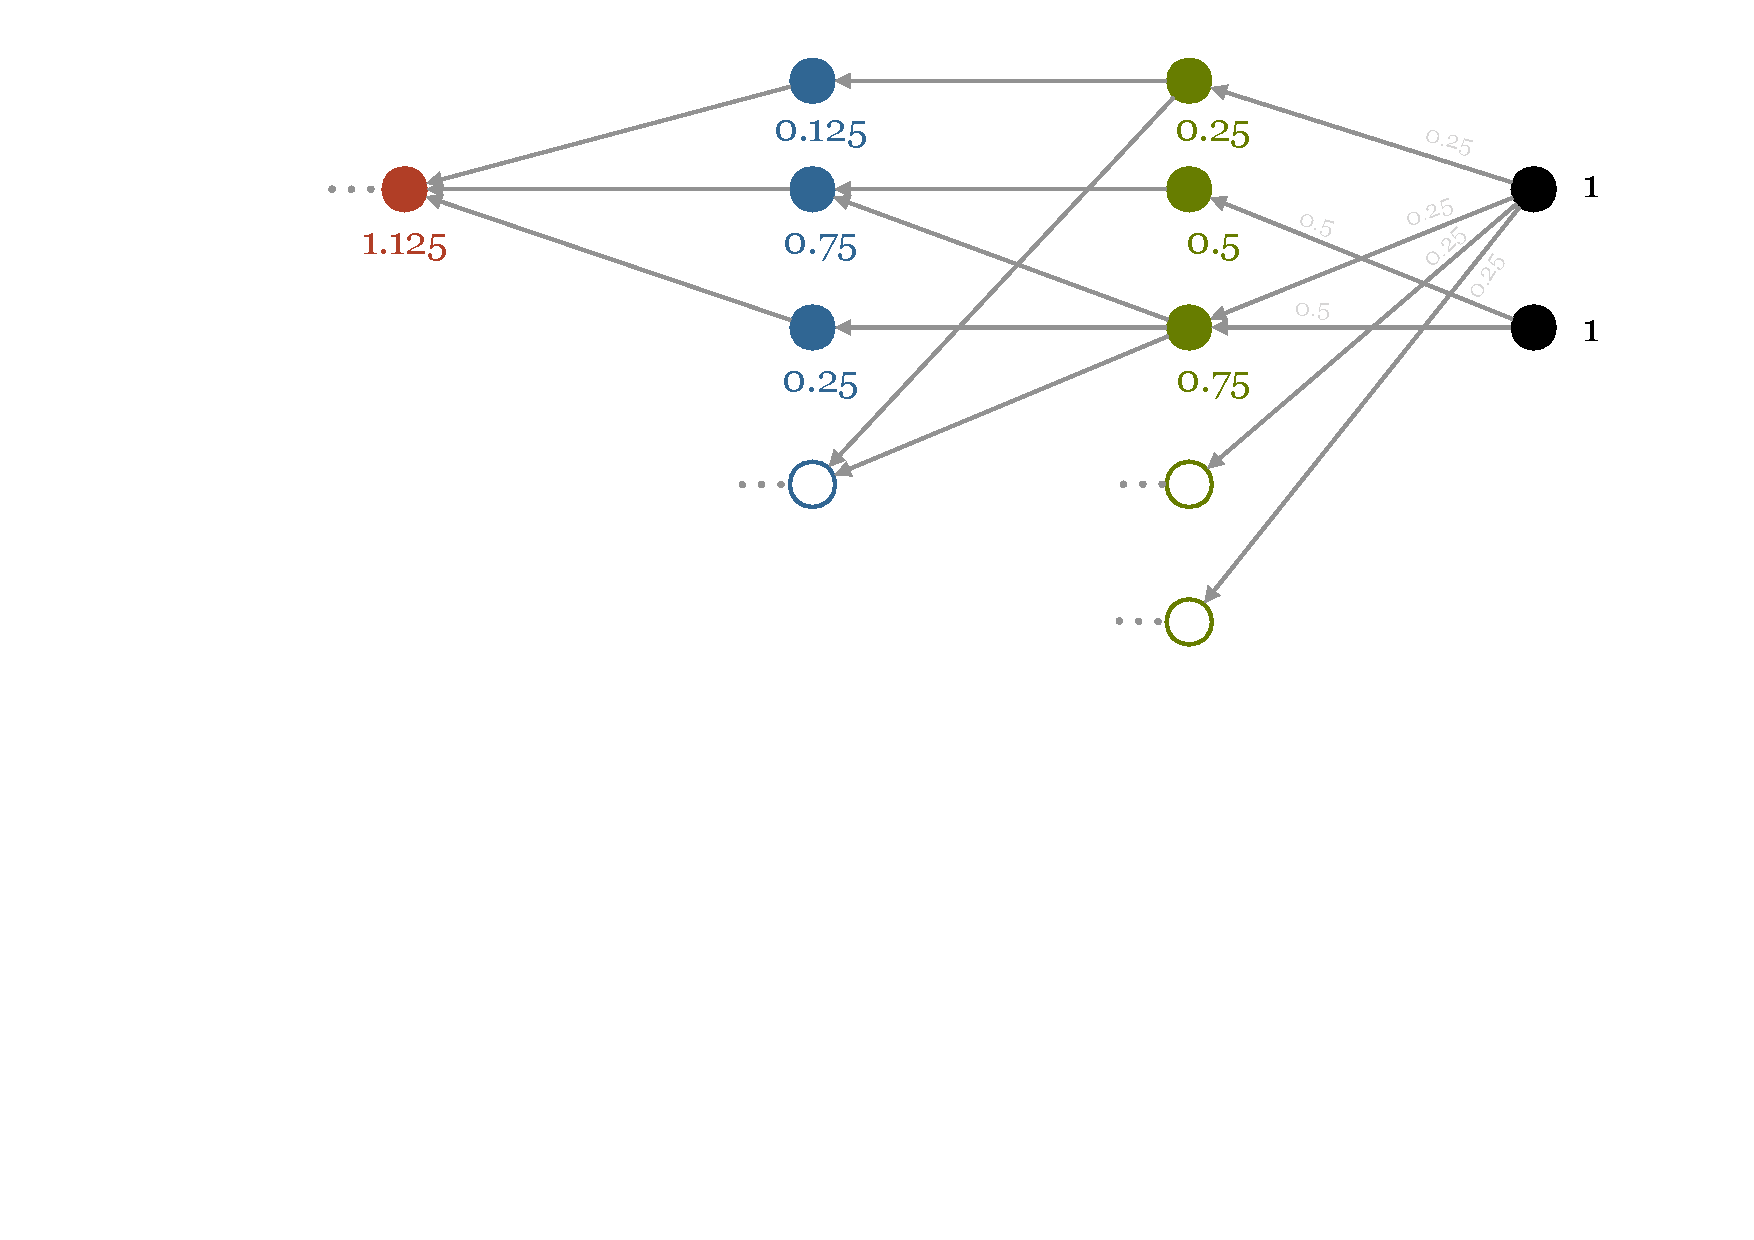
\includegraphics[width=0.9\textwidth]{./images/pca-5/backward.pdf}
	}
	\caption*{Computing the reputation for a site (the \rc{red node} on the far left). We follow all incoming links to a certain depth. At that point we assign every node we find a reputation of 1. We can then use this to determine the reputation of the nodes to which they link. We do this by distributing the 1 unit of reputation equally over all outgoing links (including the ones, indicated by open discs, that don't ultimately lead to the site we want to compute the reputation for). This gives us the reputations of the green nodes, from which we can compute the reputations of the blue nodes, which finally gives us the reputation of the red node.
	}
\end{figure}

%<figure class="narrow centering">
%<img src="/images/pca-5/backward.svg" >
%<figcaption>Computing the reputation for a site (the <span class="rc">red node</span> on the far left). We follow all incoming links to a certain depth. At that point we assign every node we find a reputation of 1. We can then use this to determine the reputation of the nodes to which they link. We do this by distributing the 1 unit of reputation equally over all outgoing links (including the ones, indicated by open discs, that don't unltimately lead to the site we want to compute the reputation for). This gives us the reputations of the green nodes, from which we can compute the reputations of the blue nodes, which finally gives us the reputation of the red node. 
%</figcaption>
%</figure>

This may seem like a slightly mind-bending idea at first, but that is mostly because we're working backwards. We can define the same idea forwards. Let's say that we start out by giving every website one unit of reputation for free. Then, at every step, every website takes all its current reputation, divides it up equally over all websites it links to and gives it all away. If the website receives no incoming links from others it is now out of reputation and stays at 0. If, however, it gets some incoming links as well as outgoing links, it also gets some new reputation. We then iterate this process: every step each website divvies up all reputation it has an gives it all away.

\begin{figure}[H]
	\centerline{
		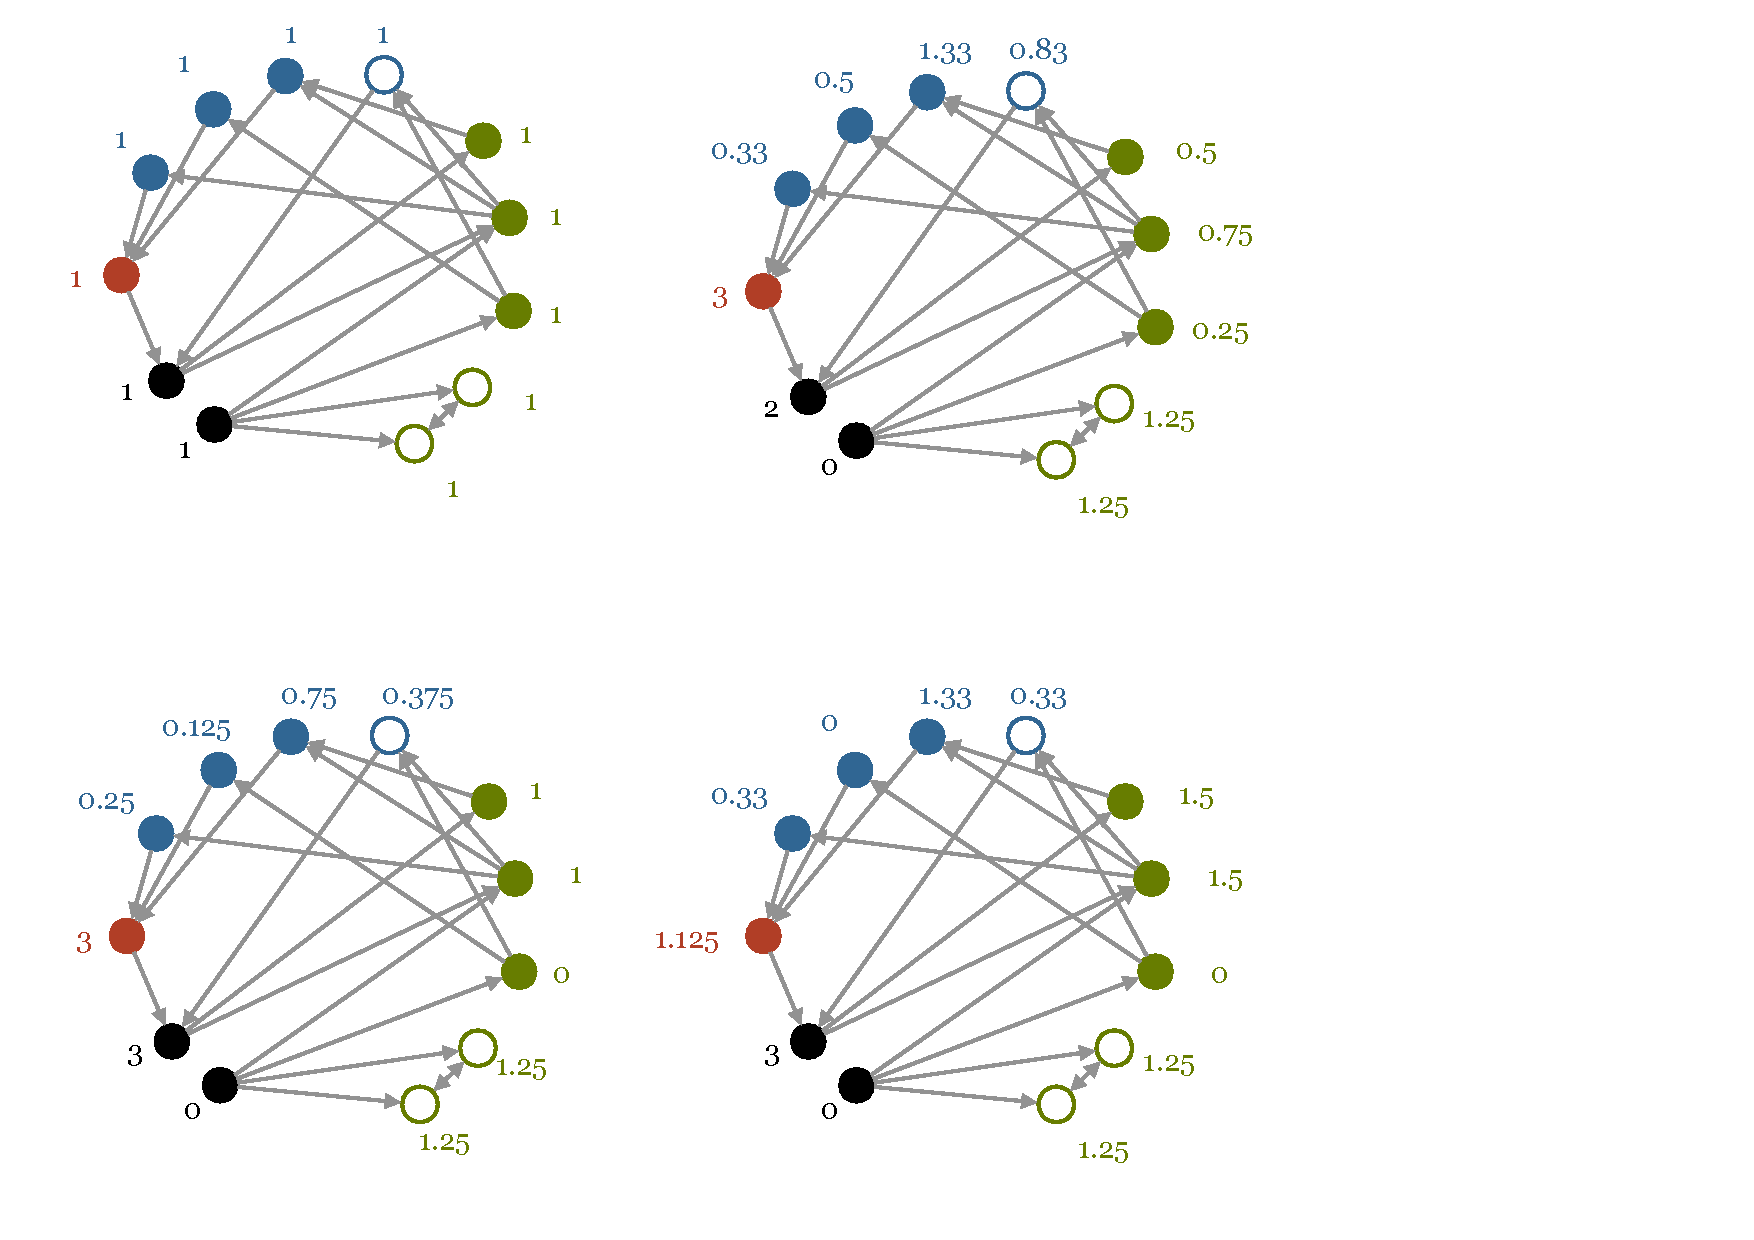
\includegraphics[width=1.1\textwidth]{./images/pca-5/forward.pdf}
	}
	\caption*{The forward computation of the reputation. We start with a reputation of 1 for every site, and have each site distribute all its reputation equally to all sites it links to. Note that after three steps, we have the same reputation for the \rc{red site} (the leftmost node in each graph).

	}
\end{figure}

%<figure class="narrow centering">
%<img src="/images/pca-5/forward.svg" >
%<figcaption>The forward computation of the reputation. We start with a reputation of 1 for every site, and have each site distribute all its reputation equally to all sites it links to. Note that after three steps, we have the same reputation for the <span class="rc">red site</span> (the leftmost node in each graph).
%</figcaption>
%</figure>

In this example, the reputations still fluctuate, and we get different values, depending on how long we continue the algorithm. However, as we will show later, for most graphs, this process eventually converges to a stable state. Each site ends up sending out as much reputation as it receives. This is the amount that we ultimately take as the reputation of the website.

Why is this hard to game? Imagine setting up a bunch of websites that all link to each other. Say you have the resources to host 10 sites. That means that at the start of the process, you get ten units of reputation. The best you can do to maintain this reputation is never to link out to legitimate websites, so no reputation flows out. But then, unless you get people to link to you, there's no reputation flowing in either.

\begin{aside}The two open green nodes in the graph above are an example of this. They claim a bit of the reputation at the start, but they aren't linked to by the rest of the network, where there is much more reputation flowing around.
\end{aside}

Compare this to a site like Wikipedia, or BBC News. Each of their pages will be linked to by hundreds of sites, each of which will themselves have high reputation. You'd need to set up at least hundreds of thousands of websites to equal that amount of reputation.

What does any of this have to do with eigenvectors? The link becomes clear when we try to figure out what the stable state of this process is. Given a particular graph of websites and who links to whom, what's the ultimate amount of reputation each site ends up with?

First we need to translate the problem setting to linear algebra. Let's say we have a set of \(n\) websites. We can represent the directed graph of which site links to which other site (the \emph{web graph}) as a large \(n \times n\) matrix \(\bc{\mbA}\): the \emph{adjacency matrix of the web graph}.

\index{Web graph}\index{Adjacency matrix}


\begin{figure}[H]
	\centerline{
		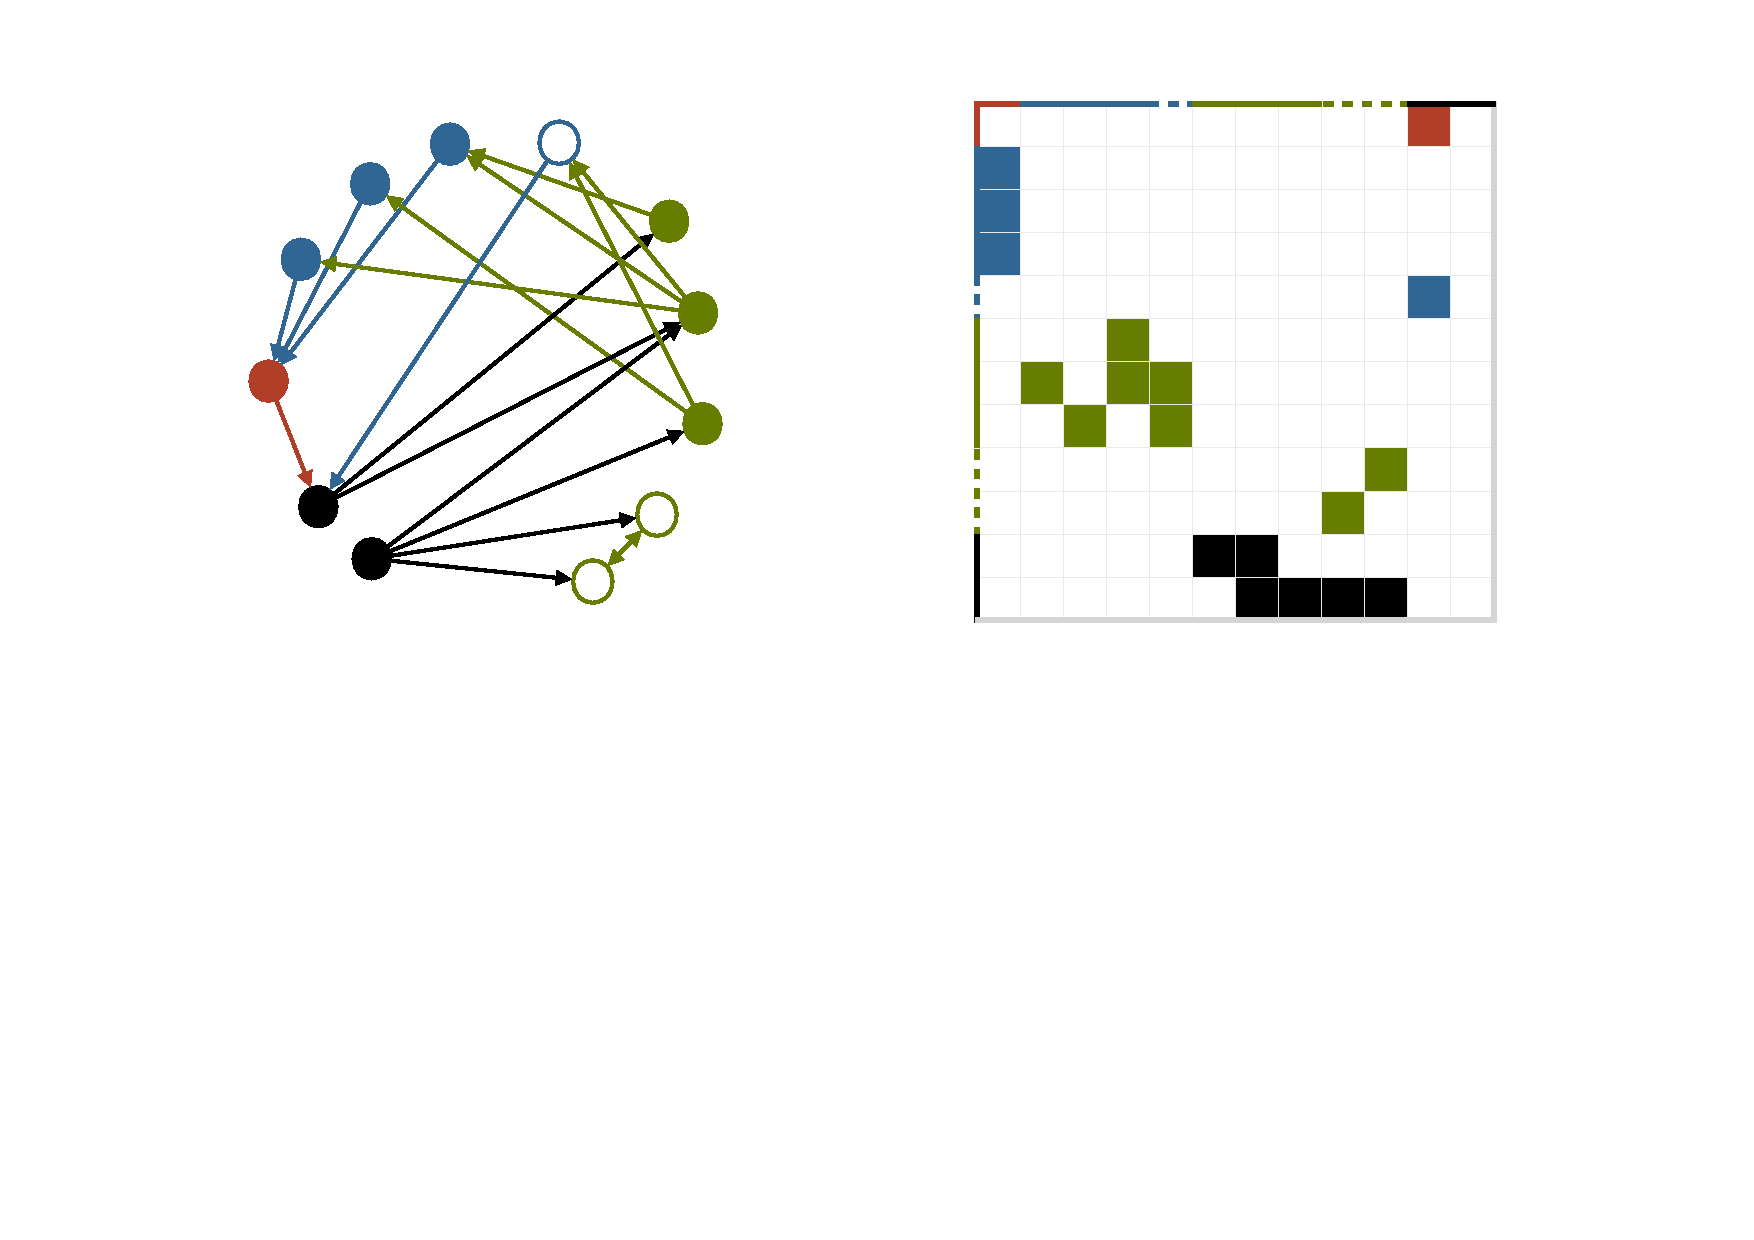
\includegraphics[width=0.9\textwidth]{./images/pca-5/adjacency.pdf}
	}
	\caption*{The adjacency matrix for our graph. Colored elements are valued 1, and white elements are valued 0. The colors only indicate the mapping to the graph, the matrix itself is just a square, binary matrix.
	}
\end{figure}

%<figure class="narrow centering">
%<img src="/images/pca-5/adjacency.svg" >
%<figcaption>The adjacency matrix for our graph. Colored elements are valued 1, and white elements are valued 0. The colors only indicate the mapping to the graph, the matrix itself is just a square, binary matrix.
%</figcaption>
%</figure>

\begin{aside}We're simplifying the problem by ignoring the fact that there can be many links between two sites and that a website (i.e. a domain) can have many different pages. If you're building a search engine, you can use all this information to make your method more powerful and more complex, but we're only interested in the basic idea here.	
\end{aside}


We can model the way website \(i\) distributes its initial unit of reputation, by starting with a \emph{one-hot vector} indicating that website. This is a vector of length \(n\), for \(n\) websites, with zeroes everywhere, except at the index \(i\), corresponding to the website \(i\), where it contains a \(1\). This represents our starting point for website \(i\), where it has one unit of reputation, and hasn't distributed anything yet.

If we multiply this vector by our adjacency matrix, we end up with a new vector that contains \(1\)'s for all the websites that \(i\) linked to.

However, this doesn't keep the total amount of reputation fixed. To keep the sum total amount of reputation in the system constant, the website should break its one unit of reputation into \(k\) equal parts, and give each to one of the \(k\) sites it links to. As a simple solution, we \emph{normalize} the vector after the multiplication: we compute the sum of all the elements in the vector and then divide each by the sum.

\begin{aside}We could also normalize the adjacency matrix \(\bc{\mbA}\) over the rows, but separating the two steps will serve to illustrate an important point later.
\end{aside}

Now, we can just repeat the process. We multiply the vector by \(\bc{\mbA}\), normalize it, multiply the result by \(\bc{\mbA}\) again, and so on. Every time we iterate this algorithm, the reputation \emph{diffuses} across the graph a little more.

\index{Matrix multiplication!iteration of}

\begin{figure}[H]
	\centerline{
	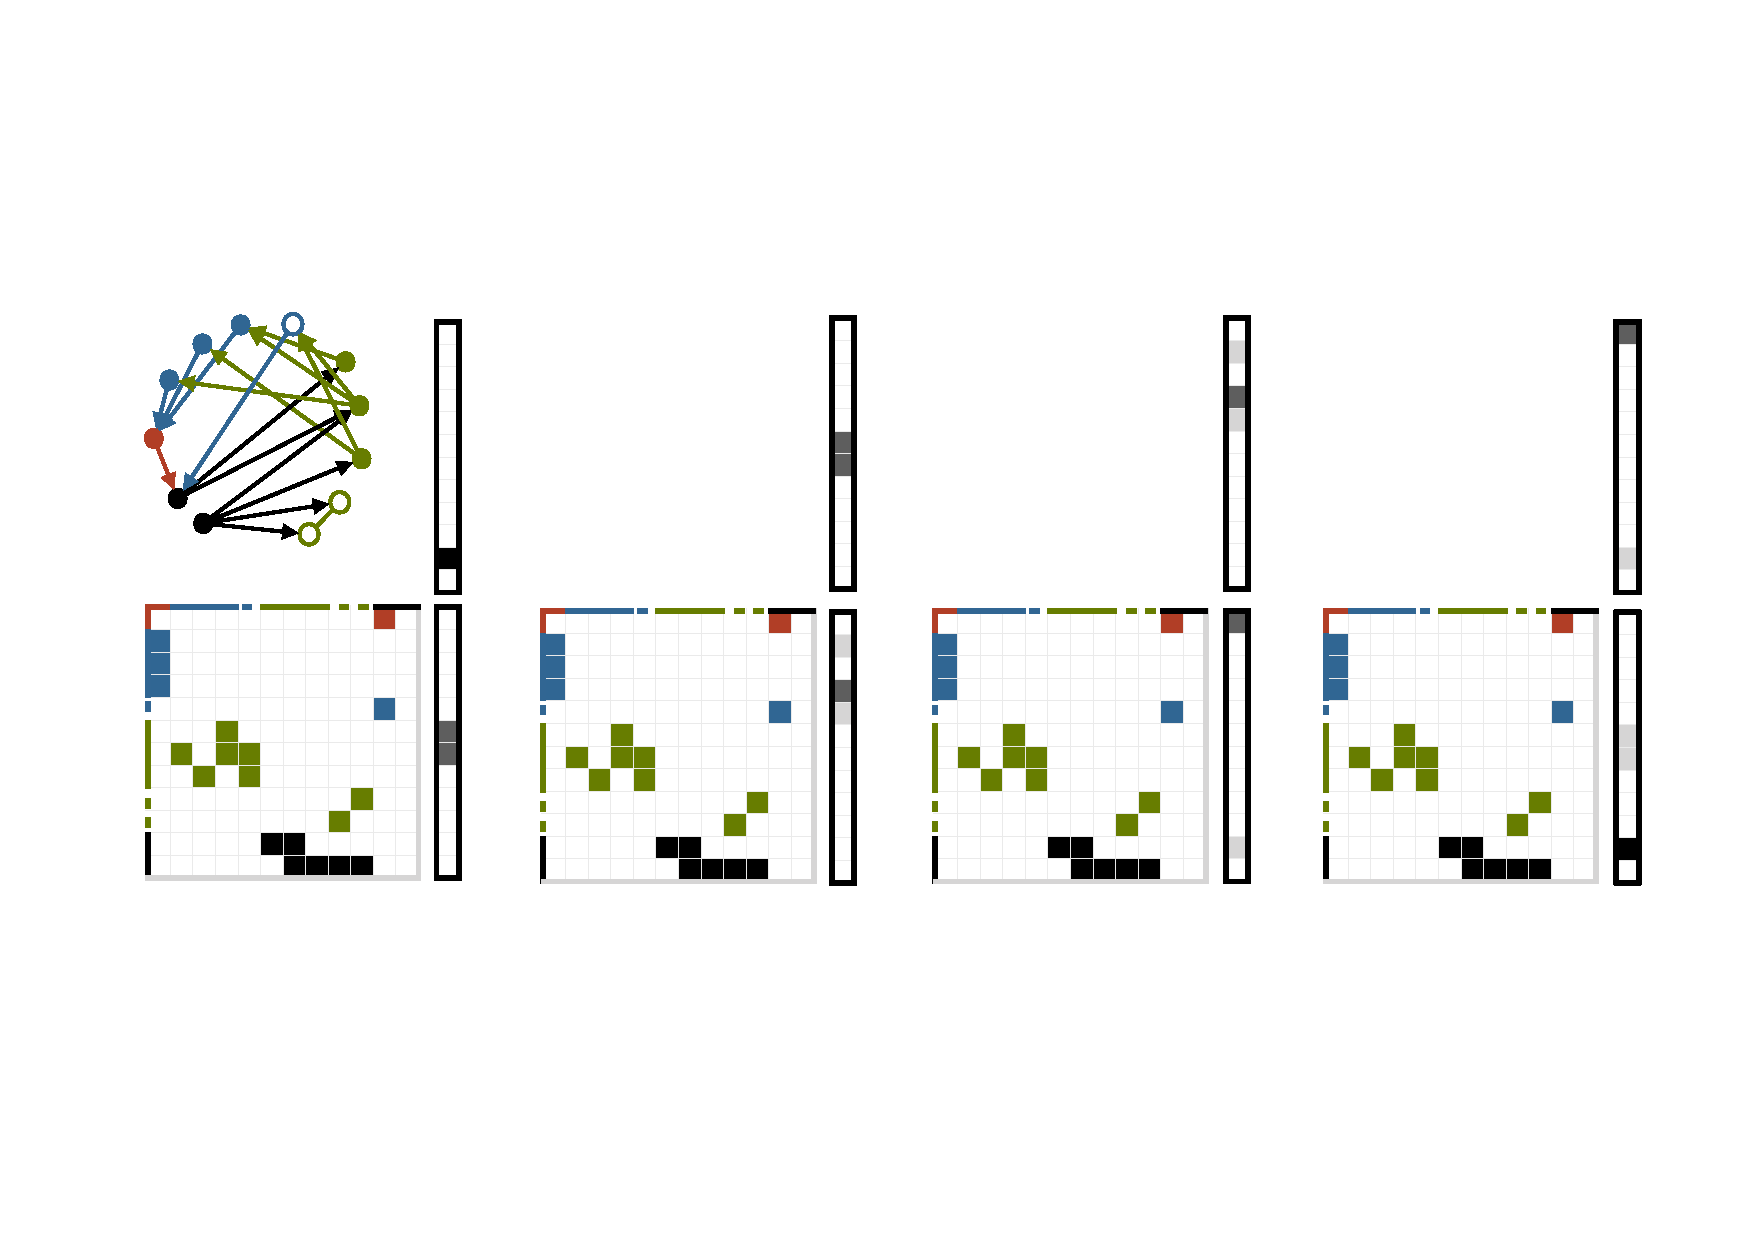
\includegraphics[width=1.1\textwidth]{./images/pca-5/matrix-it.pdf}
	}
	\caption*{Multiplying a one-hot vector by the adjacency matrix, and normalizing, allows us to see how one node's unit of reputation diffuses across the network. After four iterations, most of its reputation has circled back, but some of it has spread to other nodes. Eventually this iteration will converge to a stable vector.
	}
\end{figure}

%<figure class="narrow centering">
%<img src="/images/pca-5/matrix-it.svg" >
%<figcaption>Multiplying a one-hot vector by the adjacency matrix, and normalizing,   allows us to see how one node's unit of reputation diffuses across the network. After four iterations, most of its reputation has circled back, but some of it has spread to other nodes. Eventually this iteration will converge to a stable vector.
%</figcaption>
%</figure>

What ultimately happens to this sequence of vectors depends on the properties of the graph. However, for most graphs, especially the slightly messy ones like the web graph, the process will converge to a fixed state. For most almost all starting vectors, this multiplication will lead ultimately to a single vector, which when multiplied by the adjacency matrix, and normalized, \textbf{remains the same}. It doesn't matter what site we start at, we will always end up with the same distribution of reputation across the graph.

And that provides the link with eigenvectors. If we call the input input vector \(\rc{\mbv}\) and the factor required to normalize the result of the matrix multiplication \(\frac{1}{\bc{\lambda}}\), then we have reached a stable state when:

\begin{align*}
\frac{1}{\bc{\lambda}}\bc{\mbA}\rc{\mbv} &= \rc{\mbv} \\
\bc{\mbA}\rc{\mbv} &= \bc{\lambda}\rc{\mbv} \p
\end{align*}

This should look familiar. It's the definition of an \emph{eigenvector}, which we first saw in Chapter~\ref{chapter:eigenvectors}. If we reach a stable state, we have found a vector for which multiplying it by \(\bc{\mbA}\) changes its length, but not its direction. In short, if we try this iterative approach, and it converges, \emph{we have found an eigenvector of our matrix}. In fact, as we will see in a bit, we will have found the \emph{first} eigenvector. The one with the largest eigenvalue.

\begin{aside}For me, this is probably the key intuition for why eigenvectors are so important. If we iterate the operation of the matrix, the eigenvectors represent stable states (ignoring changes in magnitude). The key to eigenvectors is that when you want to characterize an operation, you start with its stable states.\end{aside}

In Google's use case, this tells us that after infinitely many redistributions of reputation, the distribution of reputation over the web stabilizes. This is the basic idea behind \emph{pagerank}, Google's main algorithm (at least in the early days). The websites that ultimately end up with the most reputation, are likely to provide quality content and should end up higher in the ranking of the search results.

\index{Pagerank|)}

You may wonder why all the reputation doesn't flow into a single website. This \emph{could} happen if a website is linked to, but doesn't link anywhere else. The real pagerank algorithm includes a few tricks to avoid such situations, but so long as a website has incoming and outgoing links, it will end up with some proportion of the reputation, but not all of it, the same way a bathtub with the tap running and the plug removed will never be fully empty.

We can extend this principle to a lot of other situations. In any process where some quantity---like reputation, money or people---is distributed between entities according to fixed proportions, the final, stable state of such a system is an \emph{eigenvector} of the matrix describing how the quantitiy is redistributed.

For instance, if you have a number of cities, and some statistics describing what proportion of people move from every city to every other city for each year, you can work out what populations the cities will stabilize to.

\begin{aside}\href{https://setosa.io/ev/eigenvectors-and-eigenvalues/}{This explainer of eigenvalues} by Victor Powell and Lewis Lehe provides a nice tool to visualize just this scenario.
\end{aside}

In these examples, the quantity being redistributed was reputation, or population. We can also take this quantity to be \emph{probability}. Instead of counting the total number of people in each city, we can take the probability that a single person moving around randomly, ends up in a given city after some fixed, large number of steps \(n\).

Or, in the Google example, imagine a user starting at a given website \(i\), and clicking a random outgoing link. We don't observe which link they click, so the best we can say is that the user is on one of the sites that \(i\) links to, with each getting equal probability. That is, we get a uniform distribution over all websites linked to by \(i\). This is exactly the vector that we get from one iteration of our algorithm: we multiply the one-hot vector for \(i\) by \(\bc{\mbA}\) and normalize.

If the user, wherever they've ended up, clicks another random link, our distribution representing their current position diffuses again. If we had a probability of \(0.1\) for them being on website \(j\), and \(j\) links out to two other websites, each of these gets probability \(0.05\). All we need to do is multiply the probability vector by \(\bc{\mbA}\) again, and normalize.

This kind of description of a linear redistribution of quantities is called a \emph{Markov process} or a \emph{Markov chain}. It's a very useful branch of mathematics, but we'll not dig into it any deeper. It has provided us with two things. First, another perspective on eigenvectors as the stable states to which the process of repeated matrix multiplication converges. Second, \emph{a way of computing at least one eigenvector}.

This bring us back to the business at hand. How do we compute eigenvectors?

%<!--
%As we saw in [part two](/blog/pca-2), the principal components of a mean-centered dataset are the eigenvectors of the covariance matrix. If we estimate this covariance matrix from the data, all we need to do is find its eigenvalues.
%
%<aside>As shown in <a href="/blog/pca-2">part two</a>, the covariance matrix for mean-centered data \(\X\) can be estimated with \(\X^T\X\) divided by the number of instances \(N\) (or \(N-1\) for an unbiased estimate).</aside>
% -->

Let's follow the iteration approach and analyse it a bit more carefully. When we compute the eigenvectors of the covariance matrix \(\bc{\mbS}\), we have two advantages over Google. First, the matrix we will deal with is probably much smaller than the adjacency matrix of the web graph. We'll assume that we can easily store it in memory and multiply vectors by it. Second, since it's a covariance matrix, \emph{we know that it's symmetric}. This will make several aspects of our analysis a lot simpler.

The algorithm suggested by the story of Google can be summarized by the following iteration:

\[
\mbx \leftarrow \frac{\bc{\mbA}\mbx}{\|\bc{\mbA}\mbx\|_1} \p
\]

That is, we multiply \(\bc{\mbA}\) by \(\mbx\) and then divide the entries of the resulting vector by its sum, which we've denoted here by the L1-norm \(\|\cdot\|_1\).

As it turns out, it doesn't matter much what norm we normalize by. We can just as easily use the Euclidean norm, and normalize the vector to be a unit vector after each step. If we do this, it stops being a probability vector, but the algorithm still yields an eigenvector. Since it makes the analysis a little simpler, we'll switch to that approach, and use the iteration

\[
\mbx \leftarrow \frac{\bc{\mbA}\mbx}{\|\bc{\mbA}\mbx\|} \p
\]

If we removed the normalization step, and made the iteration \(\mbx \leftarrow \bc{\mbA}\mbx\), it would be very easy to see that after a number of iterations, say four, the resulting vector \(\mbx_4\) would be \(\bc{\mbA}\bc{\mbA}\bc{\mbA}\bc{\mbA}\mbx_0\), where \(\mbx_0\) is the vector we started with. Put simply, we would have \(\mbx_k = \bc{\mbA}^k \mbx_0\).

Luckily, the normalization step doesn't make things much more difficult than this. Note that the norm of a vector is a \emph{linear quantity}: if we multiply all the elements of the vector by 2, the norm is also multiplied by 2. In short \(\|\mbx\bc{c}\| = \|\mbx\|\bc{c}\).
%
%<!-- <aside>This is a standard property in geometry: if you scale a figure, and one line segment is scaled up by \(s\), then all other line segments are also scaled by \(s\). So, if the components of \(\x\) are scaled by 2, the length of \(\x\) itself is scaled by 2 as well.</aside> -->

\pagebreak\noindent Therefore, we can say that

\[
\mbx_2 = \frac{\bc{\mbA}\mbx_1}{\|\bc{\mbA}\mbx_1\|}
= \frac{\bc{\mbA}   \frac{   \bc{\mbA}\mbx_0  }{   \|\bc{\mbA}\mbx_0\|}  }{   \|\bc{\mbA}\frac{   \bc{\mbA}\mbx_0  }{   \|\bc{\mbA}\mbx_0\|}\|}
= \frac{ ~\, \bc{\mbA}\bc{\mbA}\mbx_0   \;\;\frac{1}{ \|\bc{\mbA}\mbx_0\|}  }{   \| \bc{\mbA}\bc{\mbA}\mbx_0 \|\frac{1}{   \|\bc{\mbA}\mbx_0\|}} = \frac{\bc{\mbA}^2\mbx_0}{\|\bc{\mbA}^2\mbx_0\|} \p
\]

Or, more generally, the \(k\)-th vector in our iteration is just the vector \(\bc{\mbA}^k\mbx_0\), normalized. We can normalize every iteration, every other iteration or every \(k\) iterations. The end result will be the same. 

\begin{aside}That is, unless the values get so big they can no longer be stored accurately in floating point representation. That's why in practice, it pays to normalize every iteration.
\end{aside}

Let's see what we can say about this vector \(\bc{\mbA}^k\mbx_0\).

First, we know from the spectral theorem that if \(\bc{\mbA}\) is \(n \times n\) and symmetric, it has \(n\) real eigenvalues \(\bc{\lambda}_i\)---including multiplicities---and \(n\) corresponding eigenvectors \(\rc{\mbv}_i\). We'll assume that the eigenvalues are sorted by magnitude, so that \(\bc{\lambda}_1\) is the biggest eigenvalue, and \(\bc{\lambda}_2\) the second biggest, and so on.

We also know, from previous chapters, that the eigenvectors form a basis: any vector in \(\mR^n\) can be written as a linear combination of the eigenvectors. That means that we can write \(\mbx_0\) as \(c_1\rc{\mbv}_1 + \;\ldots\; + c_n\rc{\mbv}_n\), for some values \(c_1 \;\ldots\;  c_n\). If we choose \(\mbx_0\) randomly, the probability that any of these are exactly \(0\) will be vanishingly small.

%<!--
%<aside>In mathematical parlance, we say this is "almost certain", or that it has probability 1. In practice, this isn't quite true once we start implementing the algorithm on an actual computer, but the probability is small enough.
%</aside>
% -->

Now, let's see what we get if we start with \(\mbx_0\) written like this, and compute \(\mbx_k\). First, let's look at the unnormalized vector \(\bc{\mbA}^k\mbx_0\)

\begin{align*}
\bc{\mbA}^k\mbx_0 &= \bc{\mbA}^k(c_1\rc{\mbv}_1 + c_2\rc{\mbv}_2 + \;\ldots\; + c_n\rc{\mbv}_n) \\
&=c_1\bc{\mbA}^k\rc{\mbv}_1 + c_2\bc{\mbA}^k\rc{\mbv}_2 + \;\ldots\; + c_n\bc{\mbA}^k\rc{\mbv}_n \\
&=c_1{\bc{\lambda}_1}^k\rc{\mbv}_1 +  c_2{\bc{\lambda}_2}^k\rc{\mbv}_2 + \;\ldots\; + c_n{\bc{\lambda}_n}^k\rc{\mbv_n} \\
&=c_1{\bc{\lambda}_1}^k \left(\rc{\mbv}_1 +  \frac{c_2}{c_1}\frac{{\bc{\lambda}_2}^k}{{\bc{\lambda}_1}^k}\rc{\mbv}_2 + \;\ldots\; + \frac{c_n}{c_1}\frac{{\bc{\lambda}_n}^k}{{\bc{\lambda}_1}^k}\rc{\mbv}_n \right ) \p \\
\end{align*}

In the last line, we take the factor \(c_1{\bc{\lambda}_1}^k\) out of the brackets. This leaves the term \(\rc{\mbv}_1\) by itself, and divides the rest of the terms by this factor. Note the factors \({\bc{\lambda}_i}^k/{\bc{\lambda}_1}^k\) in all terms except the first. We know that \(\bc{\lambda}_1\) is the eigenvalue with the greatest magnitude, so \(\bc{\lambda}_i/\bc{\lambda}_1\) is always in the interval \([-1, 1]\). This means that its \(k\)-th power goes to zero with \(k\). For large enough \(k\), all that remains is

\[
\bc{\mbA}^k\mbx_0 \to c_1{\bc{\lambda}_1}^k \rc{\mbv}_1 \p
\]

That is, we converge to the first eigenvector. We can now add the normalization back in, but that doesn't affect the direction of the vector we end up with, only its magnitude. 

\begin{aside}This analysis also tells us the rate of convergence. Every iteration, the second biggest term in our sum decays with a factor of \(|\bc{\lambda}_2/\bc{\lambda}_1|\). This tells us that we are converging geometrically, and that the speed of convergence is determined by the difference in magnitude between the biggest and the second biggest eigenvalue.
\end{aside}

This is the method of \textbf{power iteration}. A very simple way of computing eigenvectors and a very powerful one. All you need is a way to compute matrix/vector products and a way to normalize your vectors. Even on something as large as the web adjacency matrix, this is a feasible computation, (if you store the matrix in the right way).

\index{Power iteration|textbf}

\subsection{Orthogonal iteration: adding another eigenvector}

\index{Orthogonal iteration}
\index{Computing eigenvectors!by orthogonal iteration}

So, that's a simple way to compute the dominant eigenvector. What do we do if we need more eigenvectors? The simplest trick is to use the fact that \textbf{eigenvectors are always orthogonal to one another}.

Let's try a simple approach: we perform the power iteration to make our vector \(\mbx\) converge to the dominant eigenvector, but at the same time, we also perform the power iteration on a second vector \(\mby\) orthogonal to \(\mbx\). After each iteration, \(\mbx\) and \(\mby\) won't necessarily be orthogonal anymore, so we explicitly change \(\mby\) to be orthogonal to \(\mbx\) after every step.

How do we force one vector \(\mby\) to be orthogonal to another \(\mbx\)?  The simplest way to achieve this, is to first project \(\mby\) onto \(\mbx\), call the result \(\bc{\mby_\mbx}\), and then to assume that \(\mby\) consists of two components: the part \(\bc{\mby_\mbx}\), that points in the same direction as \({\mbx}\) and the remainder \(\rc{{\mby}_r}\). This tells us that \({\mby} = \bc{{\mby}_x} + \rc{{\mby}_r}\), and thus that \(\rc{\mby_r} = {\mby} - \bc{{\mby}_\mbx}\).


\begin{figure}[H]
  \centerline{
    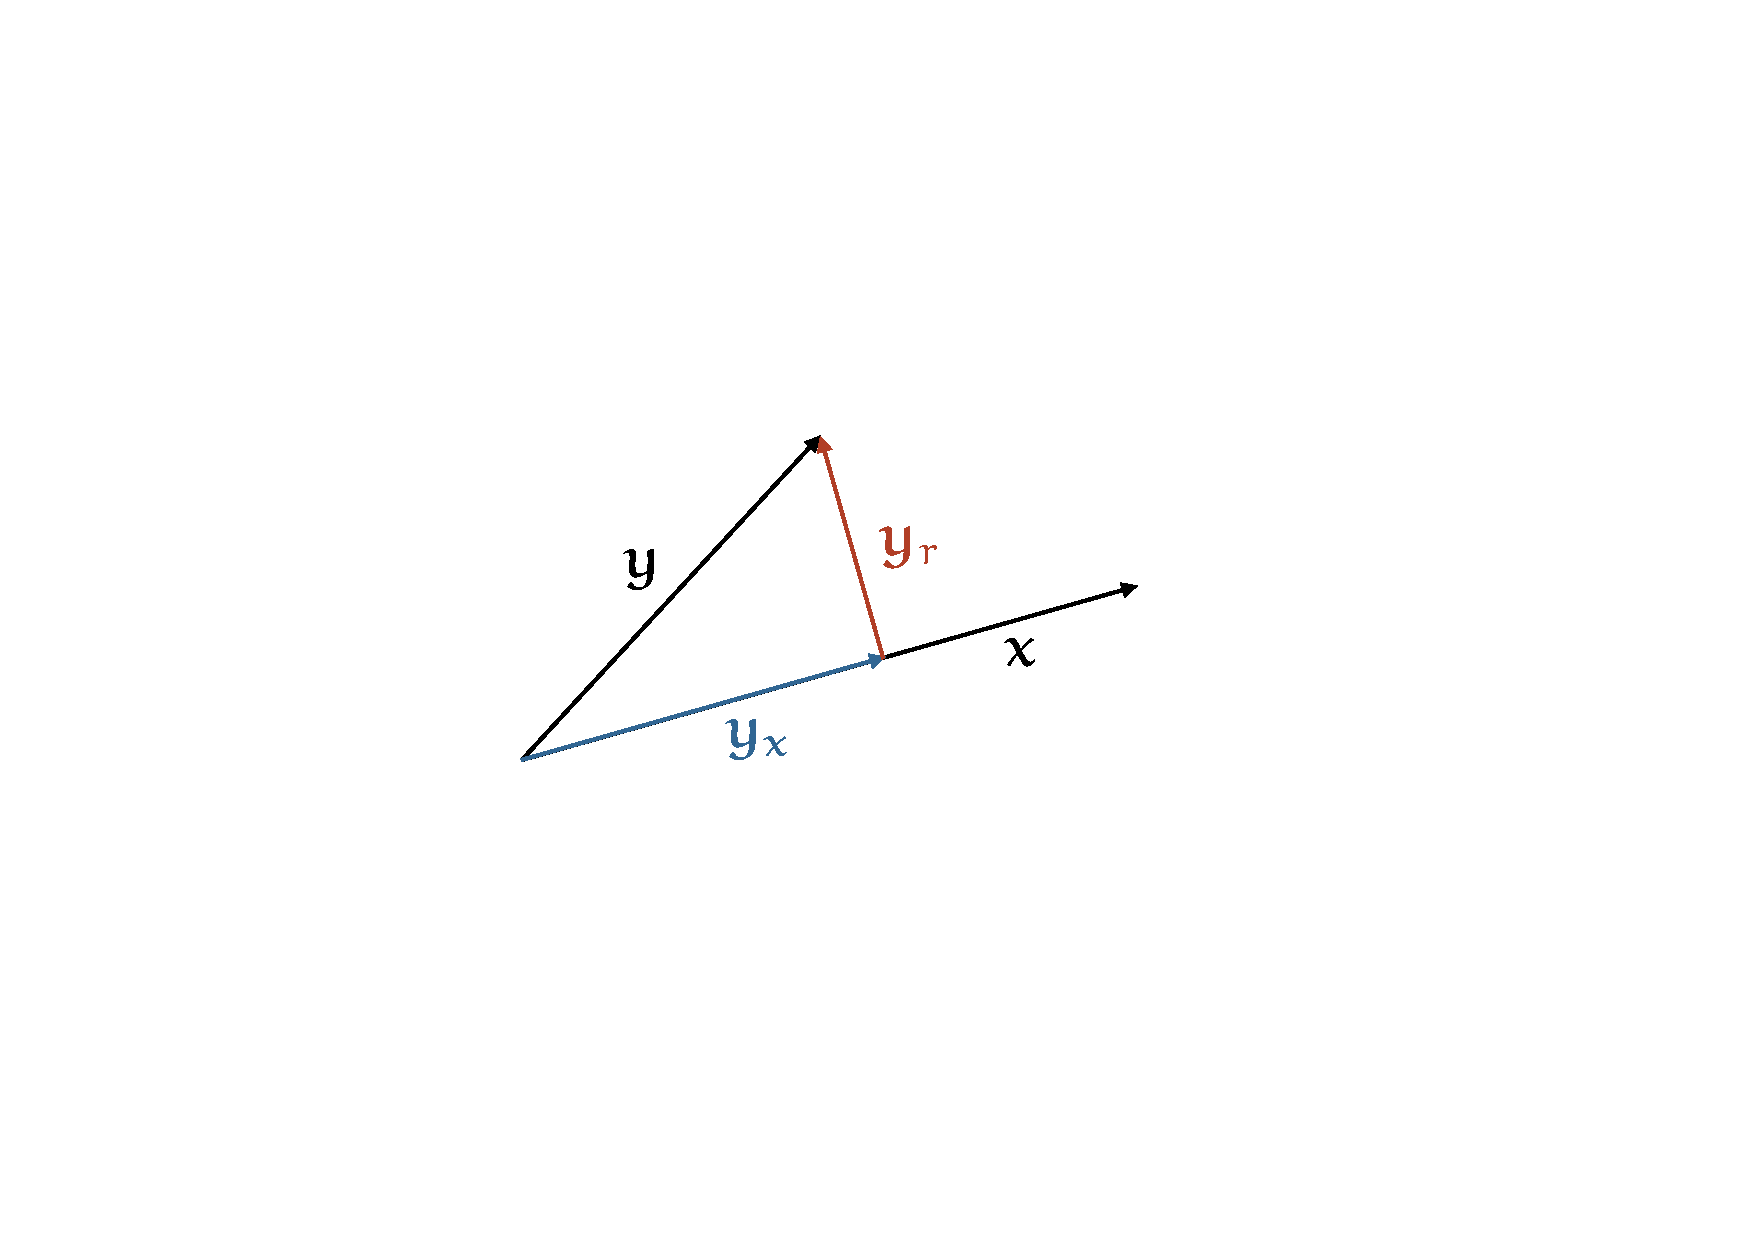
\includegraphics[width=0.7\textwidth]{./images/pca-5/rejection.pdf}
  }
\end{figure}

%<figure class="narrow centering">
%<img src="/images/pca-5/rejection.svg" class="half" >
%</figure>

The vector \(\rc{\mby_r}\), \({\mby}\) minus \bc{\(\mby\) projected onto \({\mbx}\)} is called the \emph{rejection} of \({\mby}\) from \({\mbx}\). We'll use this to build our new power iteration. Here is the new algorithm:

\begin{align*}
&\textbf{loop:} \\
&\tab {\mbx}, {\mby} \leftarrow \bc{\mbA}{\mbx}, \bc{\mbA}{\mby} & \\
&\tab {\mby} \leftarrow {\mby} - \bc{\mby_\mbx} & \text{make \({\mby}\) orthogonal to \({\mbx}\)} \\
&\tab {\mbx}, {\mby} \leftarrow {\mbx}/\|{\mbx}\|,\; {\mby}/\|{\mby}\| & \text{normalize both}
\end{align*}

Note that the operations we apply to \(\mbx\) are exactly the same as before. All we've done is to add another vector to the iteration. Our earlier proof that \(\mbx\) converges to the dominant eigenvector \(\rc{\mbv}_1\) still applies to this algorithm. The question is, what does \(\mby\) converge to?

Intuitively, it seems like a good bet that \(\mby\) will convergence to the second most dominant eigenvector. To help us analyze this question, and to build a foundation for later algorithms, we'll first take this algorithm and rewrite it in matrix operations.

The first line is easy: if we create a new \(n \times 2\) matrix \([\;\mbx\;\mby\;]\) with vectors \(\mbx\) and \(\mby\) as columns, then the matrix multiplication \(\bc{\mbA}[\;\mbx\;\mby\;]\) gives us a new \(n \times 2\) matrix whose columns are the new \({\mbx}\) and \({\mby}\). 

The second and third line, rejection and normalization, we can actually represent in a single matrix operation called a \emph{QR decomposition}. A QR decomposition takes a rectangular matrix \(\mbZ\) and represents it as the product of a rectangular matrix \(\rc{\mbQ}\) whose columns are all mutually orthogonal unit vectors, and a square matrix \(\mbR\) which is upper triangular (all values below the diagonal are \(0\)).

\index{QR decomposition|textbf}

To apply this to our algorithm, let \(\mbZ \leftarrow \bc{\mbA}[\;\mbx\;\mby\;]\), the \(n \times 2\) matrix we create in the first line. If we apply a QR decomposition \(\mbZ = \rc{\mbQ}\mbR\), then \(\rc{\mbQ}\) must be an \(n \times 2\) matrix with 2 orthogonal unit vectors for columns, and \(\mbR\) must be a \(2 \times 2\) matrix with the bottom-left element \(0\).

If we draw a picture, it becomes clear that what lines 2 and 3 of our algorithm are doing is computing a QR decomposition of \(\mbZ\).

\begin{figure}[H]
  \centerline{
    \hspace{3em}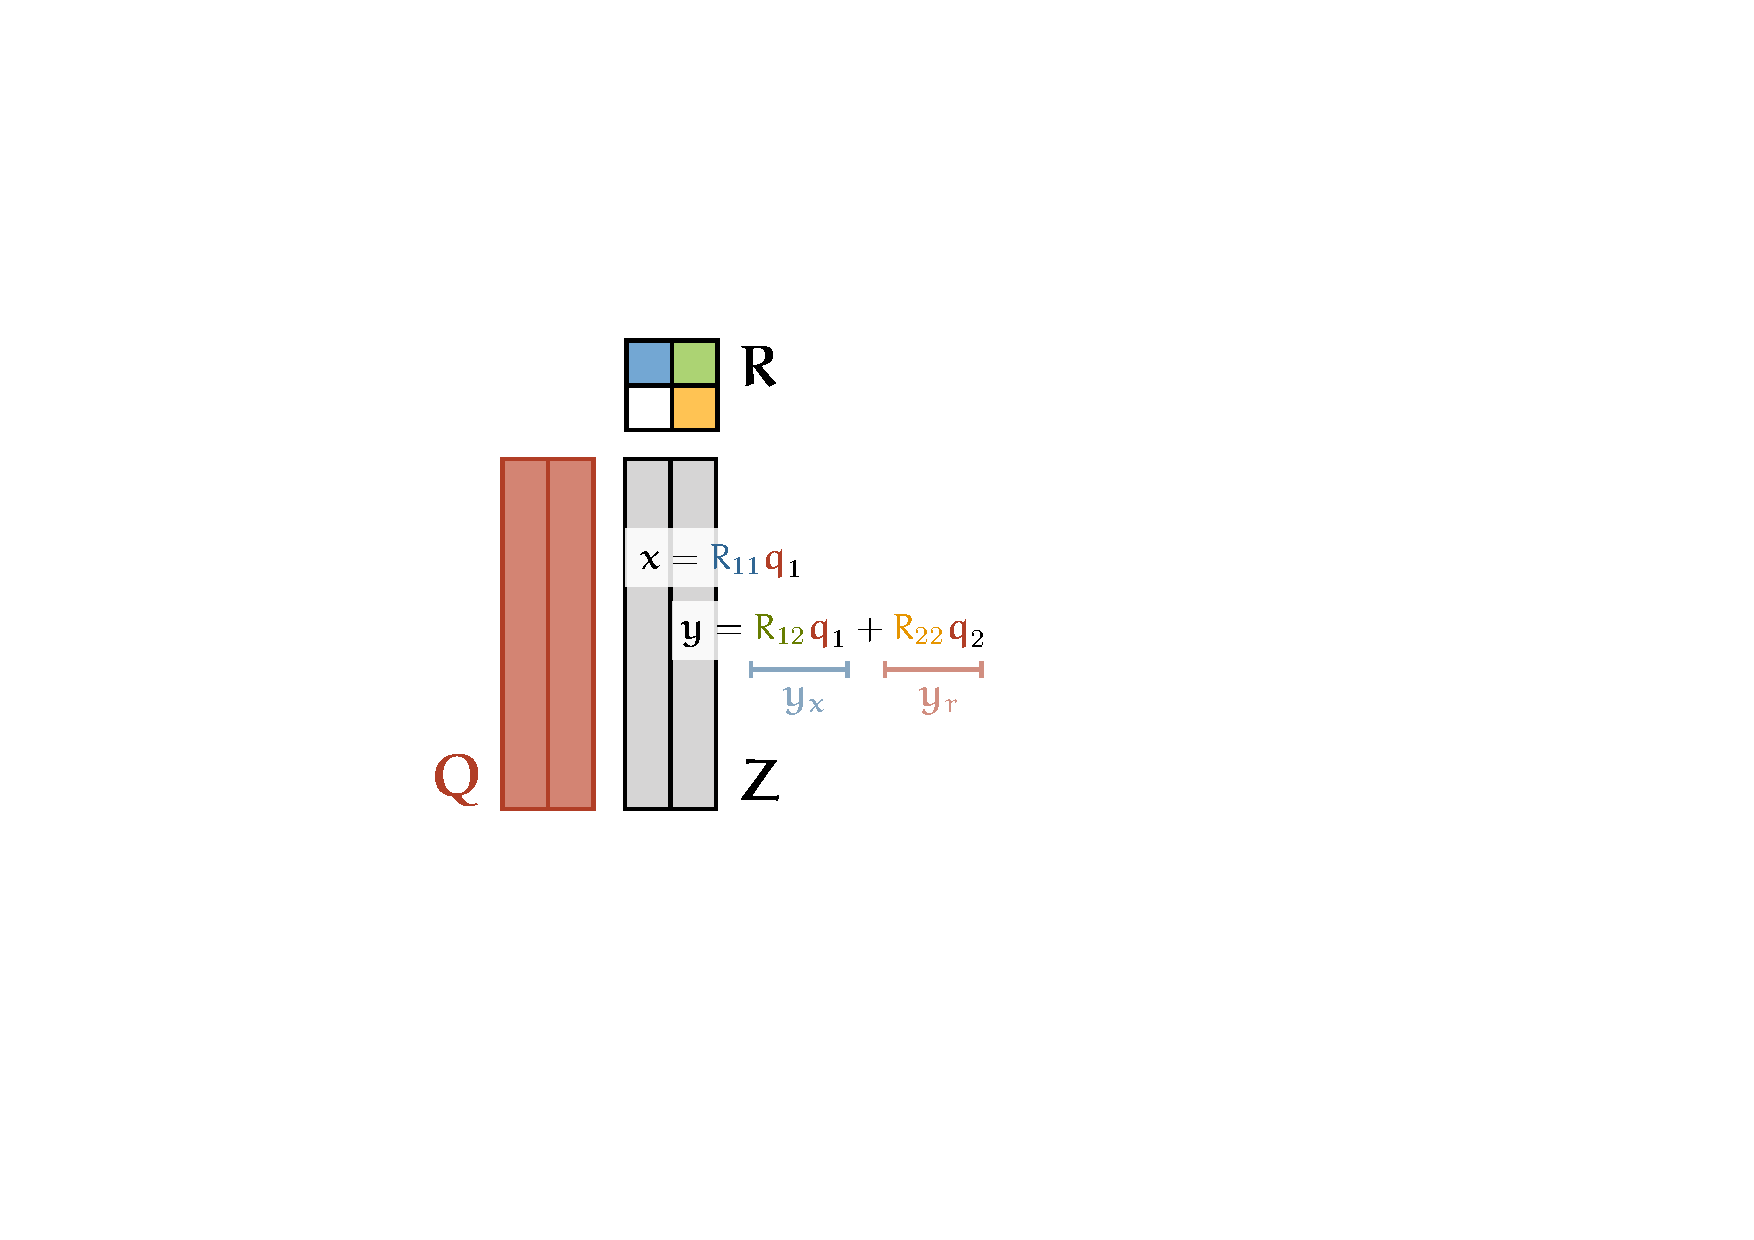
\includegraphics[width=0.7\textwidth]{./images/pca-5/two-column-qr.pdf}
  }
  \caption*{The QR decomposition of a matrix with two columns.}
\end{figure}

%<figure class="narrow centering">
%<img src="/images/pca-5/two-column-qr.svg" class="half">
%<figcaption>The QR decomposition of a matrix with two columns.
%</figcaption>
%</figure>

Because \(\mbR\) is upper triangular, the first column of \(\mbZ = \rc{\mbQ}\mbR\) is just the first column of \(\rc{\mbQ}\) multiplied by some scalar. Because we require the first column of \(\rc{\mbQ}\) to be a unit vector, this must be the scalar that normalizes the first column of \(\mbZ\).

The second column of \(\mbZ\) is a linear combination of the two columns of \(\rc{\mbQ}\). Here the requirement we get from the definition of the QR decomposition is that the second column of \(\rc{\mbQ}\) is also a unit vector, \emph{and} that it is orthogonal to the first column. As we worked out above, this requires us to subtract the projection of \(\mby\) onto \({\mbx}\) from the original \({\mby}\) before we normalize.

With this perspective, we can rewrite our algorithm as

\begin{align*}
&\rc{\mbQ} \leftarrow \left[\;\mbx_0 \; \mby_0\;\right] \\
&\textbf{loop:} \\
&\tab \mbZ \leftarrow \bc{\mbA}\rc{\mbQ} & \\
&\tab \rc{\mbQ}, \mbR \leftarrow \text{qr}(\mbZ) \p\\
\end{align*}

%with the columns of \(\rc{\mbQ}\) converging to the eigenvectors \(\rc{\mbv}_1\) and \(\rc{\mbv}_2\).

Let's see what happens to the second vector \({\mby}\) under our iteration. As before, the key is to note that \(\bc{\mbA}\) has eigenvectors \(\rc{\mbv}_1, \ldots, \rc{\mbv}_n\) which form a basis for \(\mR^n\). That means that for our starting vector \(\mbx_0\), there are scalars \(c_1, \ldots, c_n\) so that

\[\mbx_0 = c_1\rc{\mbv}_1 + \ldots + c_n\rc{\mbv}_n\]

and similarly, for our starting vector \(\mby_0\) there are scalars \(d_1, \ldots, d_n\) so that:

\[\mby_0 = d_1\rc{\mbv}_1 + \ldots + d_n\rc{\mbv}_n \p
\]

Imagine that we set \(\mbx_0 = \rc{\mbv}_1\), and then run the algorithm. In that case the projection and rejection of \(\mby\) onto and from \(\mbx\) will look very simple. We get

\begin{align*}
\bc{\mby_\mbx} &= d_1 \rc{\mbv}_1 &&\; \kc{+} \kc{0} &&\kc{ +\;\;\ldots} && \kc{+ 0} \\
\rc{\mby_r} &= \kc{0} && \;\kc{+} d_2\rc{\mbv}_2 && + \;\;\ldots && + d_n\rc{\mbv}_n \p
\end{align*}

\begin{aside}This is simplest to see if you think of the eigenvectors as axes in which we express our vector. If we have a vector \((x, y, z)\) , then its projection onto the \(x\)-axis is simply \((x, 0, 0)\), and the corresponding rejection is \((0, y, z)\). The eigenvectors are a set of mutually orthogonal unit vectors, so we can think of them as just a different coordinate system. In this system, \(\mby\) has coordinates \((d_1, \ldots, d_n)\), so its projection onto the first eigenvector \(\rc{\mbv}_1\) is \((d_1, 0, \ldots, 0)\) and the corresponding rejection is \((0, d_2, \ldots, d_n)\).	
\end{aside}

Once we've rejected \(\rc{\mbv}_1\), we can see that multiplication by \(\bc{\mbA}\) will never result in a vector with a non-zero component in the \(\rc{\mbv}_1\) direction:
\[\bc{\mbA}\left(0\rc{\mbv}_1 + d_2\rc{\mbv}_2 + \ldots + d_n\rc{\mbv}_n\right) = \kc{0{\lambda_1}{\mbv}_1} + d_2\bc{\lambda}_2\rc{\mbv}_2 + \;\ldots\;+ d_n\bc{\lambda}_n\rc{\mbv}_n\p\]

Thus, if we start with \(\mbx_0 = \rc{\mbv}_1\), and \(\mby_0\) orthogonal to it, we have shown that under the matrix multiplication, \(\mby\) \emph{stays} orthogonal to \(\mbx\) and we can ignore the rejection step. This means we can use the same derivation as before, except that \(d_1 = 0\).


\begin{align*}
\bc{\mbA}^k\mby_0 &= \bc{\mbA}^k(d_1\rc{\mbv}_1 + d_2\rc{\mbv}_2 + c_3\rc{\mbv}_3 + \ldots + c_n\rc{\mbv_n}) \\
&= \kc{0} + d_2\bc{\mbA}^k\rc{\mbv}_2 + d_2\bc{\mbA}^k\rc{\mbv}_2 + \ldots + d_n\bc{\mbA}^k\rc{\mbv_n} \\
&= d_2{\bc{\lambda}_2}^k\rc{\mbv}_2 + d_3{\bc{\lambda}_3}^k\rc{\mbv}_3 + \ldots + d_n{\bc{\lambda}_n}^k\rc{\mbv_n} \\
&=d_2{\bc{\lambda}_2}^k \left(\rc{\mbv}_2 +  \frac{d_3}{d_2}\frac{{\bc{\lambda}_3}^k}{{\bc{\lambda}_2}^k}\rc{\mbv}_3 + \ldots + \frac{d_n}{d_2}\frac{{\bc{\lambda}_n}^k}{{\bc{\lambda}_2}^k}\rc{\mbv_n} \right ) \\
\end{align*}

Again, if the eigenvalues are all different, the factors \({\bc{\lambda}_i}^k/{\bc{\lambda}_2}^k\) for \(i>2\) all go to zero and we are left with the convergence

\[
\mby \to d_2\bc{\lambda}_2\rc{\mbv}_2 \p
\]

Essentially, we are performing the same algorithm as before, but by projecting away from \(\rc{\mbv}_1\), we are ensuring that \(\rc{\mbv}_1\) can't dominate. The next most dominant eigenvector, \(\rc{\mbv}_2\) automatically pops out.

In practice, we don't need to set \(\mbx = \rc{\mbv}_1\). The iteration on \(\mbx\) is entirely the same as what we saw in the power iteration, so we know that \(\mbx\) will converge to \(\rc{\mbv}_1\). The closer it gets, the more the \(\rc{\mbv}_1\) component of \(\mby\) will die out, and the closer the algorithm will behave to what we've described above.

This isn't quite a proof, but it hopefully gives you a sense of how the algorithm behaves when it works as it should. A more rigorous proof will be easier to give when we've extended the algorithm a bit more.

\subsection{Adding even more eigenvectors}

At this point, you can probably guess how to extend this idea to an arbitrary number of eigenvectors. For a third eigenvector, we add another vector \(\mbz\). We multiply it by \(\bc{\mbA}\) as we did with \(\mbx\) and \(\mby\), and then, we project it to be orthogonal to \emph{both} \(\mbx\) and \(\mby\). It turns out this rejection can be computed simply by subtracting from \(\mbz\) the projections onto \(\mbx\) and onto \(\mby\):

\[\rc{\mbz_r} \leftarrow \mbz - \mbz_\mbx - \mbz_y \p\]

The rest of the algorithm remains as before: we normalize all vectors, and iterate the process.

What we are essentially doing here is computing something called \emph{the Gram-Schmidt process}. For a sequence of vectors, we project the second to be orthogonal to the first. Then we project the third to be orthogonal to both the first and the projected second, and so on until we are out of vectors, normalizing each vector after computing the projections. Extending the logic of the 2 vector case, we see that the Gram-Schmidt process essentially computes a QR decomposition:

\index{Gram-Schmidt process}
\enlargethispage{4em}

\begin{figure}[H]
  \centerline{
    \hspace{4em}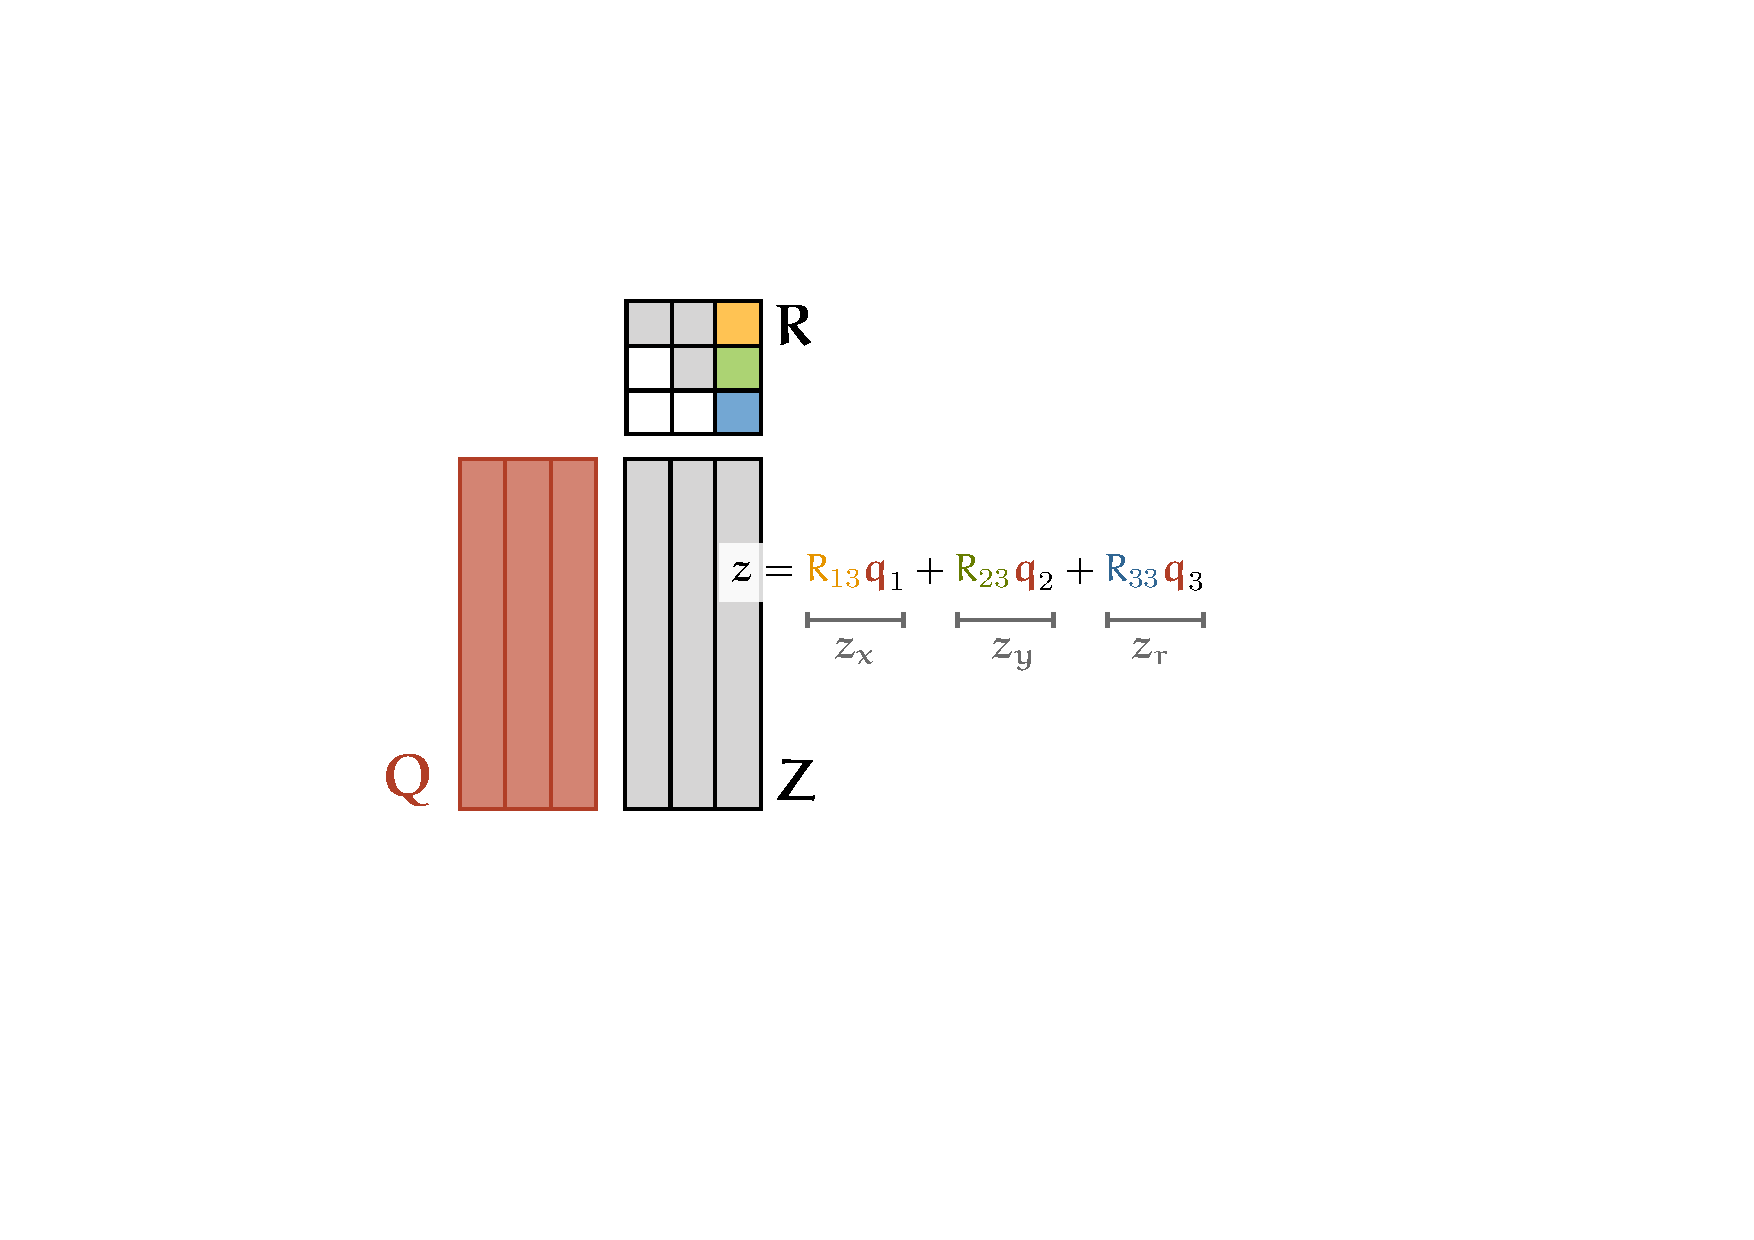
\includegraphics[width=0.7\textwidth]{./images/pca-5/three-column-qr.pdf}
  }
  \caption*{The QR decomposition of a matrix with three columns.}
\end{figure}

%<figure class="narrow centering">
%<img src="/images/pca-5/three-column-qr.svg" class="three-quarters">
%<figcaption>The QR decomposition of a matrix with three columns.
%</figcaption>
%</figure>

The resulting \(k\) mutually orthogonal vectors are the columns of \(\rc{\mbQ}\), and the \(k \times k\) matrix \(\mbR\) is the matrix such that \(\rc{\mbQ}\mbR\) results in our original matrix.

In practice, the Gram-Schmidt process isn't the most stable way to compute a QR decomposition. Most modern algorithms use a series of reflections or rotations in place of the projections that the GS process uses.

What we can show, however, is that under the right circumstances, the QR decomposition is \emph{unique}. The proof is a little technical, so we've moved it to the appendix. For now, all we need to know is that if the columns of \(\mbZ\) are linearly independent, it has exactly one QR decomposition for which all the diagonal values of \(\mbR\) are positive (which is what the Gram-Schmidt process provides). 

That means it doesn't matter how you compute it, you can analyse it as though you've computed it by the Gram-Schmidt process, which is what we'll do here.

So, to compute the first \(k\) eigenvectors, we can use the following algorithm:

\begin{align*}
&\rc{\mbQ} \leftarrow \left[\,\mbx_1 \;\ldots\; \mbx_k \,\right] \\
&\textbf{loop:} \\
&\tab \mbZ \leftarrow \bc{\mbA}\rc{\mbQ} & \\
&\tab \rc{\mbQ}, \mbR \leftarrow \text{qr}(\mbZ) \\
\end{align*}

If we use this algorithm to compute the principal components, \(\bc{\mbA}\) will be our sample covariance, so we know that we have \(n\) real eigenvalues, and we can safely set \(n = k\). In this setting, it becomes straightforward to show that when the algorithm converges, the columns of \(\rc{\mbQ}\) converge to the eigenvalues.

\begin{aside}The proof we used earlier would also work, but it pays to view things from different perspectives.
\end{aside}

To do so, we'll need to introduce a concept called \textbf{matrix similarity}. Let \(\bc{\mbA}\) be any \(n \times n\) matrix. \(\bc{\mbA}\) represents a map on \(\mR^n\). Now imagine that we have another basis on \(\mR^n\), represented by the invertible matrix \(\rc{\mbP}\): that is, we are representing the same space in a different coordinate system. In this coordinate system, our map can also be represented, but we would need a different matrix. Call this matrix \(\bc{\mbB}\).

\index{Matrix similarity}\index{Similar matrices}

What is the relation between \(\bc{\mbA}\) and \(\bc{\mbB}\)? We know that the map \(\bc{\mbA}\) should be equivalent to mapping to the basis \(\rc{\mbP}\), applying the map \(\bc{\mbB}\) and mapping back to the standard basis. Composing these operations gives us

\[\bc{\mbA} = \rc{\mbP}\bc{\mbB}\rc{\mbP}^{-1}\p\]

Any two square matrices \(\bc{\mbA}\) and \(\bc{\mbB}\) for which this relation holds---for some \(\rc{\mbP}\)---are said to be \emph{similar}. That is, they represent the same map, just in two different bases.

Similar matrices are a useful concept, because they often share many properties. Most relevant for our case, \emph{similar matrices have the same eigenvalues}. This shouldn't be a big surprise: an eigenvalue is the extent to which an eigenvector is stretched by a map. If we change our coordinate system, the direction of the eigenvector may change, but the amount by which it stretches stays the same.

\begin{aside}This does require that the origin is in the same place in both coordinate systems (as it is with a change of basis). For instance, losing 10 percent of your weight is the same in pounds or kilograms, but cooling down by 10 percent is a very different proposition in degrees Celsius than it is in kelvin.	
\end{aside}


This view of similarity also provides a new perspective on diagonalization. Remember that the spectral theorem tells us that a symmetric matrix \(\bc{\mbA}\) can be decomposed as
\index{Spectral theorem}

\[
\bc{\mbA} = \rc{\mbP}\bc{\mbD}\rc{\mbP}^T
\]

with \(\bc{\mbD}\) diagonal, and \(\rc{\mbP}\) orthogonal (implying \(\rc{\mbP}^T = \rc{\mbP}^{-1}\)). In terms of matrix similarity this simply states that every symmetric matrix is similar to some diagonal matrix. And since we can simply read the eigenvalues off the diagonal in a diagonal matrix, this is useful to know.

\pagebreak\noindent We can use the idea of matrix similarity to show that if we set \(k=n\) and the orthogonal iteration algorithm converges, it converges to a point where the columns of \(\rc{\mbQ}\) are the eigenvectors.

%<!-- 
%<aside>We've shown this already for each vector indidually, but it usually pays to show things in multiple ways. This deepens our understanding, and reduces the probability we are making mistakes or misunderstanding something.
%</aside>
% -->

First, number the sequence of \(\rc{\mbQ}\)-matrices produced by the algorithm \(\rc{\mbQ}_1\), \(\rc{\mbQ}_2\), \(\ldots\) At point \(i\) in the iteration, we know that: \(\bc{\mbA}\rc{\mbQ}_{i-1} = \rc{\mbQ}_i\mbR_i\), since that's the QR decomposition we perform at step \(i\). Because each \(\rc{\mbQ}\) is orthogonal, we can multiply both sides by its transpose, to get

\[
\bc{\mbA} = \rc{\mbQ}_i\mbR_i{\rc{\mbQ}_{i-1}}^T \p
\]

Now, if we assume that the sequence of \(\rc{\mbQ}_i\)'s and \(\mbR_i\)'s converges to some \(\rc{\mbQ}\) and \(\mbR\), in the limit the left and right \(\rc{\mbQ}\) will be the same, giving us

\[
\bc{\mbA} = \rc{\mbQ}\mbR\rc{\mbQ}^T\p
\]

This tells us that \(\bc{\mbA}\) is similar to some triangular matrix \(\mbR\). Triangular matrices, like diagonal ones, have their eigenvalues along the diagonal, so we can read the eigenvalues of \(\bc{\mbA}\) off the diagonal of \(\mbR\).

To show that \(\rc{\mbQ}\) contains the eigen\emph{vectors} of \(\bc{\mbA}\) we need another assumption: that \(\bc{\mbA}\) is symmetric: \(\bc{\mbA} = \bc{\mbA}^T\). If we know that, then we have \(\mbR = \rc{\mbQ}^T\bc{\mbA}\rc{\mbQ}\) from rewriting the similarity relationship, and \(\rc{\mbQ}^T\bc{\mbA}^T\rc{\mbQ} = \mbR^T\) from transposing both sides. Putting these together, we get:

\[
\mbR = \rc{\mbQ}^T\bc{\mbA}\rc{\mbQ} = \rc{\mbQ}^T\bc{\mbA}^T\rc{\mbQ} = \mbR^T\p
\]

Which tells us that if \(\bc{\mbA}\) is symmetric, \(\mbR\) is symmetric too, so it must be diagonal.

%<!-- 
%<aside>More technically, we can say that the orthogonal iteration converges to the Schur decomposition we saw in <a href="/blog/pca3">part 3</a>. As we noted there, if the original matrix is symmetric, the Schur decomposition becomes a diagonalization.
%</aside>
% -->

Why does this prove that \(\rc{\mbQ}\) contains the eigenvectors? Rewrite the similarity to \(\bc{\mbA}\rc{\mbQ} = \rc{\mbQ}\mbR\). This shows that multiplying \(\bc{\mbA}\) by the \(i\)-th column of \(\rc{\mbQ}\), is equivalent to multiplying it by the \(i\)-th diagonal element of \(\mbR\). This is the \(i\)-th eigenvalue, so the corresponding column of \(\rc{\mbQ}\) must be the corresponding eigenvector.

\begin{figure}[H]
  \centerline{
    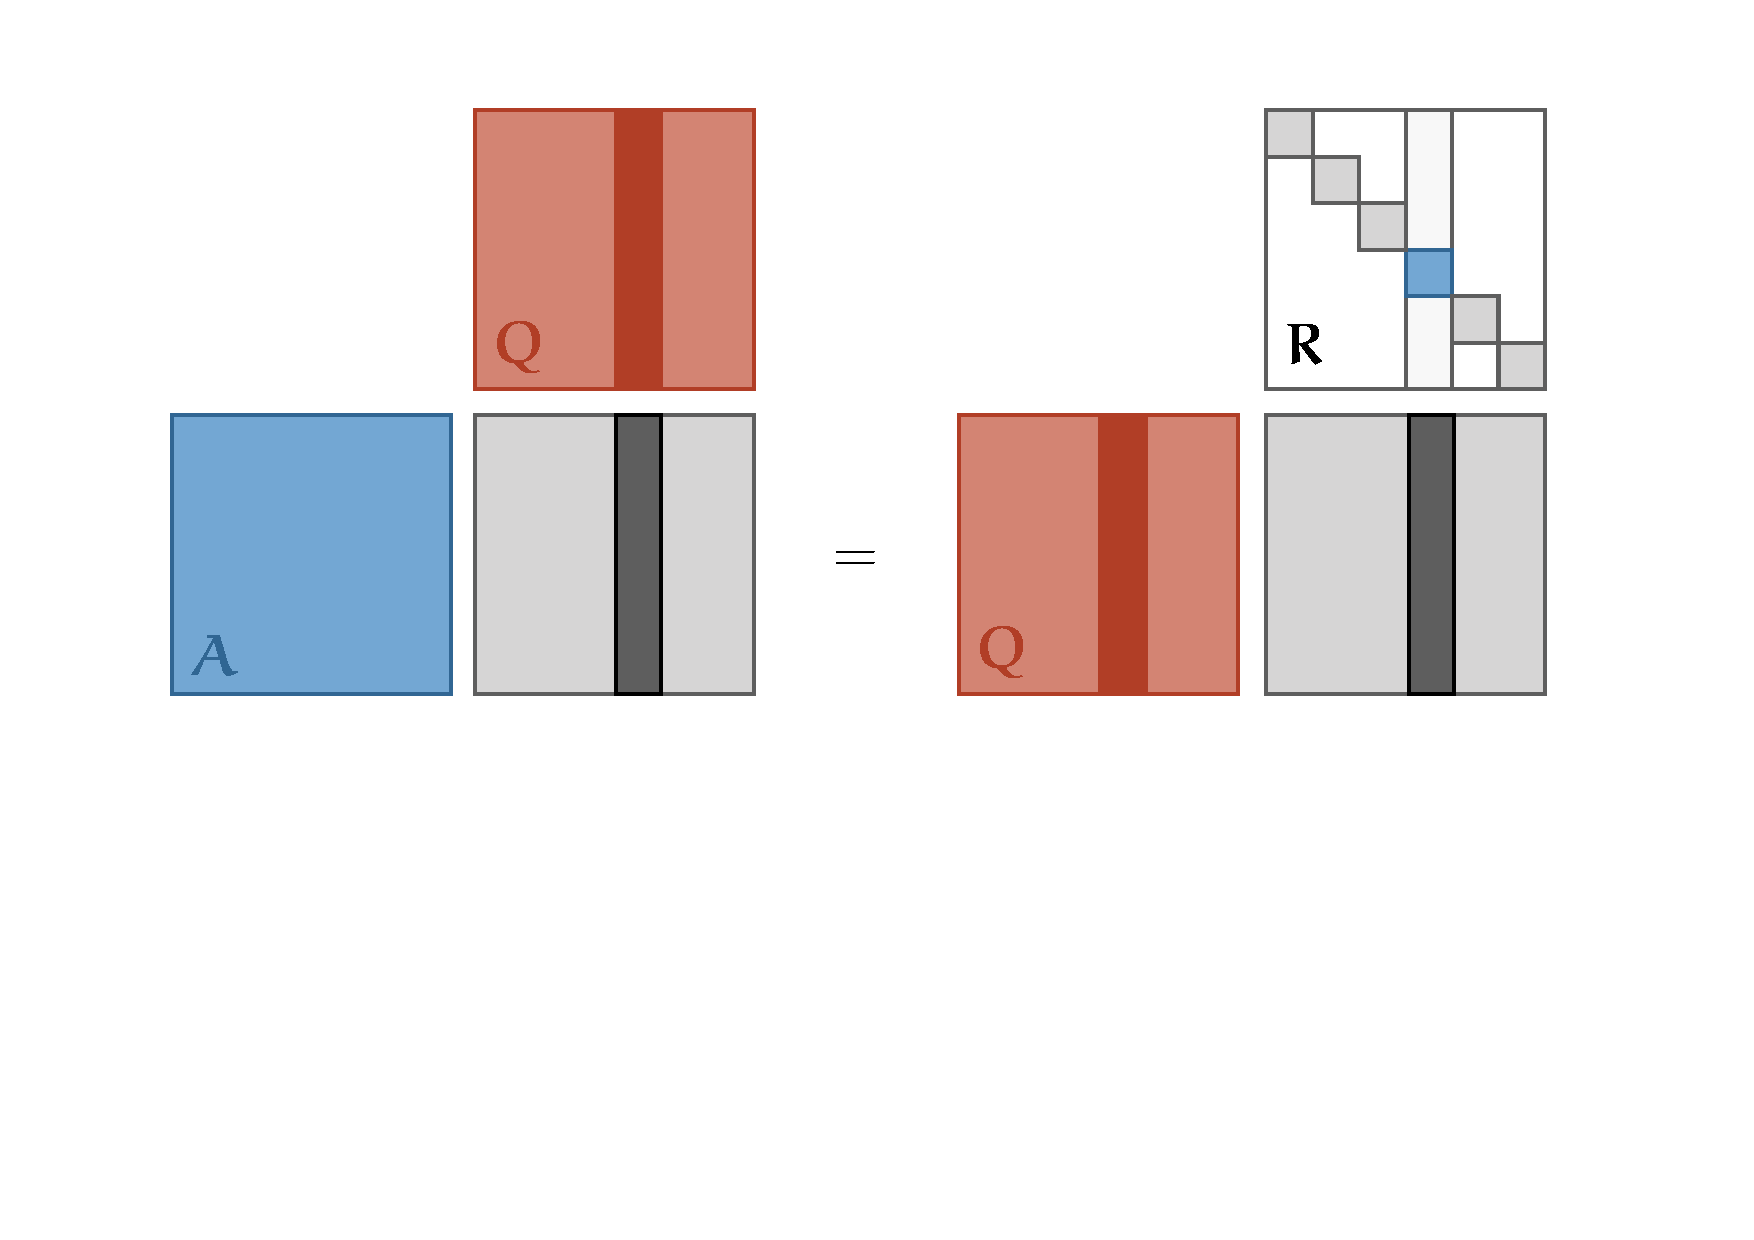
\includegraphics[width=1\textwidth]{./images/pca-5/aqqr.pdf}
  }
\end{figure}


%<figure class="narrow centering">
%<img src="/images/pca-5/aqqr.svg" class="three-quarters">
%</figure>

\subsection{QR iteration}

\index{QR iteration|textbf}
\index{Computing eigenvectors!by QR iteration}

Our final eigenvector algorithm is \emph{QR iteration}. It looks very similar to orthogonal iteration, but works slightly differently. We'll look at the algorithm first and then dig into how it works, and how it relates to the orthogonal iteration.

Here is the algorithm:

\begin{align*}
&\mbZ \leftarrow \bc{\mbA} \\
&\textbf{loop:}\\
&\tab\rc{\mbQ}, \mbR \leftarrow \text{qr}(\mbZ) \\
&\tab\mbZ  \leftarrow \mbR\rc{\mbQ} \\
\end{align*}

Note the difference in how \(\bc{\mbA}\) is used. In the orthogonal iteration, we used \(\bc{\mbA}\) in every iteration to multiply by. Here, it is only used at the very start. We compute its QR decomposition, multiply \(\rc{\mbQ}\) and \(\mbR\) in \emph{reverse order}, and iterate.

\begin{aside}This only works if both \(\rc{\mbQ}\) and \(\mbR\) are \(n \times n\). With the orthogonal iteration, we could choose how many eigenvectors we wanted to compute. With the QR iteration, we are always computing the full set.
\end{aside}

The key idea of this algorithm is that each new matrix \(\mbZ\) is \emph{similar} to the previous one. We can easily show this if we number the sequence \(\mbZ_0\), \(\mbZ_1\), \(\ldots\) and similarly for the \(\rc{\mbQ}\)'s and \(\mbR\)'s. We then have

\begin{align*}
\mbZ_{i} &= \mbR_i\rc{\mbQ}_i &\text{line 4 in iteration \(i\)}\\
&= {\rc{\mbQ}_{i}}^T\rc{\mbQ}_{i}\mbR_i\rc{\mbQ}_i  &\text{because } {\rc{\mbQ}_i}^T\rc{\mbQ}_i = \mbI\\
&= {\rc{\mbQ}_{i}}^T\mbZ_{i-1}\rc{\mbQ}_i & \text{line 3 in iteration \(i-1\)}\p
\end{align*}

Note the key principle: for every \(\rc{\mbQ}\) and \(\mbR\) in the sequence, \(\rc{\mbQ}\mbR\) is the previous \(\mbZ\) and \(\mbR\rc{\mbQ}\) is the next \(\mbZ\).

This tells us that the sequence of \(\mbZ\)'s we generate are all similar to one another, including to the first, which is equal to \(\bc{\mbA}\). If one of them happens to be triangular or diagonal, we can simply read the eigenvalues of \(\bc{\mbA}\) off the diagonal.

\index{Matrix similarity!in QR iteration}

To show that we eventually get such a matrix, we can show that the sequences computed by the QR iteration and the orthogonal iteration are related in a very precise way.

First, let \(\rc{\mbQ}'_1\), \(\rc{\mbQ}'_2\), \(\ldots\) and \(\mbR'_1\), \(\mbR'_2\), \(\ldots\) be the sequences computed by the \emph{orthogonal} algorithm.

\begin{aside}Note the prime to indicate that these come from the orthogonal algorithm, not the QR algorithm.\end{aside}

We know that under the right conditions, the orthogonal algorithm converges to the diagonalization \(\bc{\mbA} = \rc{\mbQ}'\bc{\mbD}{\rc{\mbQ}'}^T\), or equivalently \(\bc{\mbD} = {\rc{\mbQ}'}^T\bc{\mbA}\rc{\mbQ}'\).

Now, for every step in the sequence of the orthogonal algorithm, we will define a new matrix called the matrix \(\bc{\mbD}_i\). Its definition is 

\[\bc{\mbD}_i = {\rc{\mbQ}'_i}^T\bc{\mbA}\rc{\mbQ}'_i\p\]

Note that this is a different sequence from the intermediate values \(\mbR'_i\) computed by the orthogonal algorithm. There, we had \(\bc{\mbA} = \rc{\mbQ}'_i\mbR'_i{\rc{\mbQ}'_{i-1}}^T\) or equivalently
\[
\mbR'_i = {\rc{\mbQ}'_i}^T\bc{\mbA}\rc{\mbQ}'_{i-1} \p
\]

\(\mbR'_i\) are the values that the orthogonal algorithm computes. The sequence of \(\bc{\mbD}_i\)s is simply a sequence of new matrices we now define. We know that the sequences converge to the same point, as the difference between \(\rc{\mbQ}'_{i-1}\) and \(\rc{\mbQ}'_i\) vanishes, but early on, \(\mbR'_i\) may be very different from \(\bc{\mbD}_i\).

\begin{aside}Note also that \(\bc{\mbD}_i\) \emph{converges} to a diagonal matrix (if \(\bc{\mbA}\) is symmetric), but the intermediate values won't necessarily be diagonal.
\end{aside}

Let's look at the sequence \(\bc{\mbD}_i\) around time \(i\). For the step prior to that, \(i - 1\), we know that

\begin{align*}
\bc{\mbD}_{i-1} &= {\rc{\mbQ}'_{i-1}}^T\bc{\mbA}\rc{\mbQ}'_{i-1}   &\text{by the definition of \(\bc{\mbD}_{i-1}\)} \\
&= \rc{\mbQ}'_{i-1}\rc{\mbQ}'_i\mbR'_i& \text{since \(\bc{\mbA}\rc{\mbQ}'_{i-1}\) is QR'ed in step \(i\).}
\end{align*}

Then, at step \(i\), after the QR decomposition, \(\mbR'_i = {\rc{\mbQ}'_i}^T\bc{\mbA}\rc{\mbQ}'_{i-1}\). We can use this to write:

\begin{align*}
\bc{\mbD}_{i} &= {\rc{\mbQ}'_{i}}^T\bc{\mbA}\rc{\mbQ}'_{i}   & \\
&= {\rc{\mbQ}'_{i}}^T\bc{\mbA}{\rc{\mbQ}'_{i-1}}^T\rc{\mbQ}'_{i-1}\rc{\mbQ}_{i}  & \text{because \({\rc{\mbQ}'_{i-1}}^T{\rc{\mbQ}'_{i-1}} = \mbI\)} \\
&= \mbR'_i {\rc{\mbQ}'_{i-1}}\rc{\mbQ}'_{i} & \text{see above.} \\
\end{align*}

So, putting these together, we get
\begin{align*}
\bc{\mbD}_{i-1} &= \gc{\mbQ'_{i-1}\mbQ'_i}\mbR_i \\
\bc{\mbD}_{i} &= \mbR_i\gc{\mbQ'_{i-1}\mbQ'_i}\p
\end{align*}

Note that the factor in \gc{green} is the product of two orthogonal matrices, so itself an orthogonal matrix. This means that the first line represents a QR decomposition, with \(\rc{\mbQ} = \gc{\mbQ'_{i-1}\mbQ'_i}\).

In short, if we are given \(\bc{\mbD}_{i-1}\), we can compute \(\bc{\mbD}_i\) simply by applying a QR decomposition, and multiplying \(\rc{\mbQ}\) and \(\mbR\) in reverse order. This is precisely what the QR algorithm does.

\index{QR decomposition}

\begin{aside}In practice, the QR decomposition can be expensive to compute. There are modern versions of this algorithm that only perform the QR step implicitly, to speed up the computation.
\end{aside}

So, in the limit, we know that \(\mbZ\) converges to a matrix, which has the eigenvalues along the diagonal, and 0 everywhere else. What about the eigenvectors? You'd be forgiven for guessing that once the algorithm has converged \(\rc{\mbQ}\) contains these. That isn't the case, however. For one thing, at converge, \(\mbZ\) is diagonal, so its QR decomposition is just the identity matrix times itself.

Note what we showed earlier: that the sequence of \(\mbZ\)'s computed by the algorithm are all similar to one another. Making this explicit, we get, at iteration \(i\)
\begin{align*}
\bc{\mbD}_i = \mbZ_i &= {\rc{\mbQ}_i}^T\mbZ_{i-1}\rc{\mbQ}_i = {\rc{\mbQ}_i}^T{\rc{\mbQ}_{i-1}}^T\mbZ_{i-2}\rc{\mbQ}_{i-1}\rc{\mbQ}_{i} = \ldots \\
 &= {\rc{\mbQ}^\Pi_i}^T\bc{\mbA}\rc{\mbQ}^\Pi_i
\end{align*}

where \({\rc{\mbQ}^\Pi_i}\) is the product of all \(\rc{\mbQ}\) matrices computed so far. (Note that these are the \(\rc{\mbQ}\)s from the QR algorithm not from the orthogonal iteration.)

If the algorithm has converged to our satisfaction, \(\bc{\mbD}_i\) is diagonal and we get the required diagonalization

\[
{\rc{\mbQ}^\Pi_i}\bc{\mbD}_i{\rc{\mbQ}^\Pi_i}T = \bc{\mbA} \p
\]

The takeaway is that for this algorithm, if all you're interested in is the eigenvalues, you can run the stripped down version we presented above. If you also want the eigenvectors, you'll need to keep a running product of all the \(\rc{\mbQ}\)s you've encountered.

That concludes our three methods for computing eigenvectors of a symmetric matrix. The power iteration is a simple, and highly scalable method to find the dominant eigenvector. The orthogonal iteration is an extension we can use to add additional eigenvectors. Finally, the QR algorithm is a superficially different algorithm, that turns out to compute very a similar sequence of orthonormal bases to the orthogonal iteration.

\section{Computing the SVD}

In the previous Chapter~\ref{chapter:svd} , we did a deep dive into the singular value decomposition (SVD). The main takeaway was that this is a great way to compute the PCA, but more than that, a very versatile operation for dealing with matrices that represent any kind of data.

\pagebreak\noindent So, a fitting end to the series would be one or more algorithms for computing the singular value decomposition. Pleasingly, each of the three algorithms we saw above can be adapted to provide us with the singular vectors instead of the eigenvectors. Let's start with the simplest.

\subsection{Power iteration for the SVD}

\index{Power iteration!for the SVD}
\index{Computing SVD!by power iteration}


When we compute the eigenvectors to compute a PCA, we apply the eigenvector algorithm to the matrix \(\bc{\mbS}\). Normally, we estimate \(\bc{\mbS}\) by computing \(\mbX^T\mbX\) and dividing by the number of instances in our dataset. This division affects the eigenvalues, but not the eigenvectors, so we'll ignore that for now. Instead, we'll ask what it means to compute the eigenvectors of the matrix \(\mbX^T\mbX\).

As we saw in the previous chapter, the eigenvectors of \(\mbX^T\mbX\) are the \emph{singular} vectors of \(\mbX\). This immediately gives us an algorithm for computing singular vectors: take any rectangular matrix \(\gc{\mbM}\), compute \(\gc{\mbM}^T\gc{\mbM}\) and apply the eigenvector algorithms we developed above. 

We can fill in this \(\gc{\mbM}^T\gc{\mbM}\) and see what it tells us about the algorithm. Let's start with the power iteration. When we apply this to \(\gc{\mbM}^T\gc{\mbM}\), we get
%
\begin{align*}
&\mbx \leftarrow \mbx_0 \\
&\textbf{loop}:\\
&\tab\mbx \leftarrow \gc{\mbM}^T\gc{\mbM}\mbx \\
&\tab\mbx \leftarrow \mbx / \|\mbx\| \p
\end{align*}

If we now separate the two matrix multiplications, by \(\gc{\mbM}\) and then by \(\gc{\mbM}^T\) in two steps, we get 
%
\begin{align*}
&\mbx \leftarrow \mbx_0 \\
&\textbf{loop}\hspace{-.2em}:\\
&\tab\mby \leftarrow \gc{\mbM}\mbx \\
&\tab\mbx \leftarrow \gc{\mbM}^T\mby \\
&\tab\mbx \leftarrow \mbx / \|\mbx \| \p
\end{align*}

This is the same algorithm as before, just with the matrix multiplication separated in two steps. Next, we will add another normalization step. This changes the algorithm, but we will show that the effect is negligible.
%
\begin{align*}
&\mbx \leftarrow \mbx_0 \\
&\textbf{loop}\hspace{-.2em}:\\
&\tab\mby \leftarrow \gc{\mbM}\mbx \\
&\tab\mby \leftarrow \mby / \|\mby\| \\
&\tab\mbx \leftarrow \gc{\mbM}^T\mby \\
&\tab\mbx \leftarrow \mbx / \|\mbx\| \p
\end{align*}

This is our power iteration algorithm for the singular vectors of \(\gc{\mbM}\). Compare it to the power iteration for the eigenvectors. There, \(\bc{\mbA}\) was a \emph{map} (a square matrix): the input and output space of its transformation were the same. We simply apply the transformation, normalize and repeat. With \(\gc{\mbM}\), the input and output are different: as a result, we map a vector \(\mbx\) in the input space to a vector \(\mby\) in the output space, normalize, and then map back again by \(\gc{\mbM}^T\).

\index{Power iteration!for SVD}\index{Singular vector}

The only real change we've made from the power iteration on \(\gc{\mbM}^T\gc{\mbM}\) is the extra normalization on \(\mby\). As we did before, we can look at the result \(\mbx_2\) after two normalizations, and separate  the normalizations and matrix multiplications.

\begin{align*}
\mbx_1 &= \frac{\gc{\mbM}^T\mby}{\|\gc{\mbM}^T\mby\|} = \frac{\gc{\mbM}^T\frac{\gc{\mbM}\mbx_0}{\|\gc{\mbM}\mbx_0\|}}{\|\gc{\mbM}^T\frac{\gc{\mbM}\mbx_0}{\|\gc{\mbM}\mbx_0\|}\|} \\
& = \frac{\gc{\mbM}^T\gc{\mbM}\mbx_0}{\|\gc{\mbM}^T\gc{\mbM}\mbx_0\|} \frac{\frac{1}{\|\gc{\mbM}\mbx_0\|}}{\frac{1}{\|\gc{\mbM}\mbx_0\|}} = \frac{\gc{\mbM}^T\gc{\mbM}\mbx_0}{\|\gc{\mbM}^T\gc{\mbM}\mbx_0\|} \\
\end{align*}

Put simply, the extra normalization step doesn't change what the algorithm does: we are still computing the normalized result of \(\gc{\mbM}^T\gc{\mbM}\mbx\). All our previous proofs about the algorithm still hold. We are computing the first eigenvector of \(\gc{\mbM}^T\gc{\mbM}\), and therefore the first (right) singular vector of \(\gc{\mbM}\).

Where exactly are the singular vectors and values in this algorithm? Recall the definition: if \(\rc{\mbv}\) is a right singular vector of \(\gc{\mbM}\) and \(\rc{\mbu}\) its corresponding left singular vector, with \(\gc{\sigma}\) the corresponding singular value, then

\[\gc{\mbM}\rc{\mbv} = \gc{\sigma}\rc{\mbu} \p
\]

So, if \(\mbx\) has converged to a right singular vector of \(\gc{\mbM}\), then \(\gc{\mbM}\mbx\), after normalization, is the corresponding left singular vector. This shows that the algorithm actually gives us both singular vectors. The corresponding singular \emph{value}
 is \(\|\gc{\mbM}\mbx\|\).

\subsection{Orthogonal iteration for the SVD}
\index{Computing SVD!by orthogonal iteration}


The extension to orthogonal iteration follows very straighforwardly. As before, our intuition is that we simply take a second vector \(\mbx'\) along for the iteration, and that for the second vector---in addition to normalizing it every iteration---we make it orthogonal to \(\mbx\).

\begin{aside}We're slightly shuffling our variables here. \(\mbx'\) is the vector we previously called \(\mby\) when we extended the power iteration to multiple eigenvectors. \(\mby\) is now the intermediate variable we've introduced that results from multiplication by \(\gc{\mbM}\).
\end{aside}

To follow the spirit of the power iteration algorithm for the SVD, we do this twice: we multiply \(\mbx\) and \(\mbx'\) by \(\gc{\mbM}\), resulting in \(\mby\) and \(\mby'\). We project \(\mby'\) away from \(\mby\), so that they are orthogonal to each other, and normalize both. Then, we multiply both by \(\gc{\mbM}^T\), and again project and normalize.

The main conclusion we came to before was that we were in effect computing a QR decomposition  of the matrix \(\bc{\mbA} \left [\;\mbx \;\mbx'\;\right ]\). 

%<!-- 
%We can show that what we are doing here is computing first a QR decomposition, and then an _LQ_ decomposition. The LQ decomposition is defined in the same way as the QR decomposition, except that \(L\) is a _lower_ triangular matrix. 
% -->

For \(\gc{\mbM}\left[\;\mbx\;\mbx'\;\right]\), our logic holds the same as before: we get two orthogonal unit vectors, which can serve as the columns of \(\rc{\mbQ}\). To transform these by a \(2\times 2\) matrix \(\mbR\) so that  \(\gc{\mbM}\left[\,\mbx\;\mbx'\,\right] = \rc{\mbQ}\mbR\), the first column of \(\mbR\) only needs to stretch \(\mbx\) uniformly (it only needs a value on the diagonal). The second should express \(\gc{\mbM}\mbx'\) as two components. One component in the direction of \(\gc{\mbM}\mbx\), which gives us a scalar on the first row, and one component orthogonal to \(\gc{\mbM}\mbx\) which gives us a scalar on the second row. Therefore, \(\mbR\) is upper triangular.

\pagebreak\noindent When we apply the second step of the iteration, we start with two orthogonal unit vectors \(\mby, \mby'\) and we compute \(\gc{\mbM}^T\left [\,\mby \; \mby' \,\right]\), project and normalize. By the same logic as before, we can interpret this as another QR decomposition. For this one, we'll call the orthogonal matrix \(\rc{\mbP}\) and the upper triangular one \(\mbB\)

%<!-- 
%<p>\[
%\rc{\P}, \L = \text{qr}\left (\gc{\M}^T \left[\y \; \y' \right] \right)
%\]</p>
% -->

\[
\gc{\mbM}^T \left[\,\mby \; \mby'\, \right] = \rc{\mbP}\mbB
\]

%<!-- 
% After this step, the resulting vectors \(\x\) and \(\x'\) are orthogonal unit vectors, so we can make them the _rows_ of a \(2 \times n\) matrix \(\rc{\Q}\). If we then add a \(2 \times 2\) matrix \(\L\), requiring that \(\gc{\M}^T\left [\y \; \y'\right ]= \L\rc{\Q}\), we find that the first requires only a scalar on the diagonal, and the second requires two components, one at \(\rc{Q}_{21}\) in the direction of \(\gc{\M}\y\) and one on the diagonal.
% -->
\vspace{-2em}\enlargethispage{4em}

\begin{figure}[H]
  \centerline{
    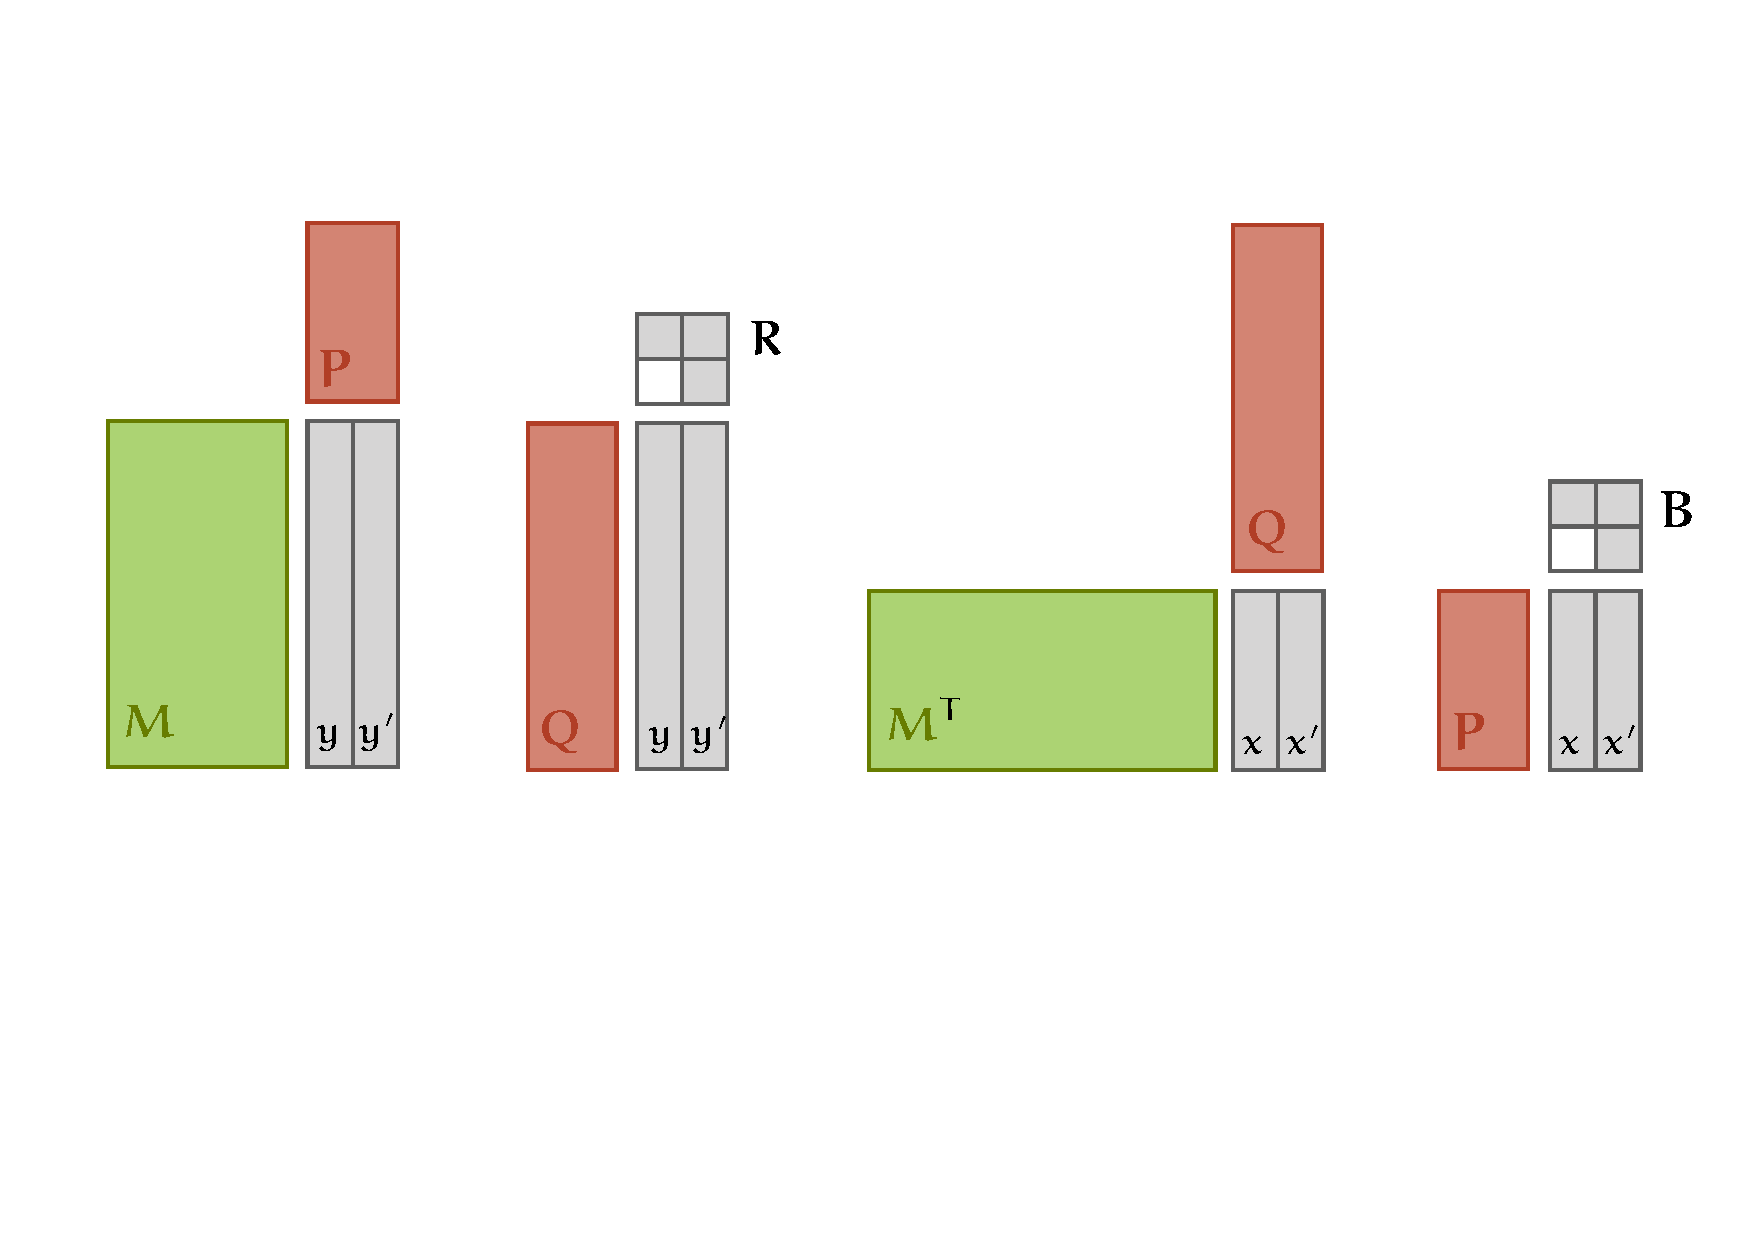
\includegraphics[width=1.1\textwidth]{./images/pca-5/orthogonal-svd.pdf}
  }
  \caption*{The two-column orthogonal algorithm for the SVD in four steps.}
\end{figure}

%<figure class="narrow centering">
%<img src="/images/pca-5/orthogonal-svd.svg" class="full">
%<figcaption>The two-column orthogonal algrithm for the SVD in four steps.
%</figcaption>
%</figure>

We can now, as before, add a third vector \(\mbx''\), a fourth, a fifth, and so on. If we make each orthogonal to all prior vectors, we end up with a matrix \(\rc{\mbQ}\) with orthogonal columns (or rows). The triangular structure of the matrix \(\mbR\) (which reverses the orthogonalization and normalization) is explained by the fact that the \(i\)-th vector has \(i\) components: \(i-1\) to describe the projections onto the previous vectors, and one to scale the remainder to a unit vector. 

\index{Orthogonalization}

Putting all of this together, we get the following algorithm to compute the first \(k\) singular vectors:

\begin{align*}
&\rc{\mbP} =\left [\,\mbx^1_0\;\ldots\;\mbx_0^k\,\right] \\
&\textbf{loop}\hspace{-.2em}: \\
&\tab \mbY \leftarrow \gc{\mbM}\rc{\mbP} \\
&\tab \rc{\mbQ}, \mbR \leftarrow \text{qr}(\mbY) \\
&\tab \mbX \leftarrow \gc{\mbM}^T\rc{\mbQ} \\
&\tab \rc{\mbP}, \mbB \leftarrow \text{qr}(\mbX) \\
\end{align*}

\begin{aside}We can also think of the second QR decomposition as an \emph{LQ decomposition} of \(\rc{\mbQ}^T\gc{\mbM}\). This follows directly from transposing both sides (The LQ decomposition gives us a lower triangular matrix and and orthogonal one). Seeing it as a QR decomposition makes more sense in the way we've explained it, but if you see this algorithm explained elsewhere, it may be with alternating LQ and QR decompositions.\end{aside}

\index{LQ Decomposition}

We know that for the first vector of \(\rc{\mbP}\), this algorithm behaves the same as the orthogonal algorithm for eigenvectors. It will converge to the first eigenvector of \(\gc{\mbM}^T\gc{\mbM}\), and therefore to the first right singular vector of \(\gc{\mbM}\).

What we haven't shown yet, is that this also holds true for the other vectors in \(\rc{\mbP}\), or for that matter, where we can find the singular values, and the left singular vectors.

In our analysis of the orthogonal algorithm for the eigenvectors, we used a simple trick: \emph{express the vectors we're iterating within the eigenbasis of the matrix}. This allowed us to see very neatly what happens as the iteration of the algorithm converges.

In the case of the SVD, we get \emph{two} bases for an \(n \times m\) matrix \(\gc{\mbM}\). One \(m \times m\) matrix \(\rc{\mbV}\) with columns \(\rc{\mbv}_1 \ldots \rc{\mbv}_m\) that spans the input space of \(\gc{\mbM}\) and one \(n \times n\) matrix \(\rc{\mbU}\) with columns \(\rc{\mbu}_1 \ldots \rc{\mbu}_n\) which spans the output space of \(\gc{\mbM}\) We'll call these the right and left \emph{singular bases} of \(\gc{\mbM}\) respectively.

\index{Singular basis}

By definition, for each of these there is a singular value \(\gc{\sigma}_i\) so that \(\gc{\mbM}\rc{\mbv}_i = \rc{\mbu}_i\gc{\sigma}_i\).

The key insight here, is that when we have the singular bases, we can express the operation of \(\gc{\mbM}\) \emph{as a mapping between them}. Each right singular basis vector is mapped onto the corresponding left singular basis vector, independent of the others.

To put this more precisely: if we express the input vector \(\mbx\) in the right singular basis \(\rc{\mbV}\), we get some an expression like
\[\mbx = c_1\rc{\mbv_1} + \;\ldots\; + c_m\rc{\mbv_k}\p\]

For every right singular vector \(i\), we get some component \(c_i\) expressing how much of \(\mbx\) projects onto \(\rc{\mbv}_i\). If we then multiply \(\mby = \gc{\mbM}\mbx\), we can express \(\mby\) in the left singular basis as:
\[\mby = d_1\rc{\mbu_1} + \;\ldots\; + d_n\rc{\mbu_k} \p\]

The key property of these two bases is that the vector \(c_i\rc{\mbv}_i\) is mapped to the vector \(d_i\rc{\mbu}_i\), \emph{independently of the other components}. We don't need to know the other values \(c_j\), the \(i\)-th component \(d_i\) is completely determined only by \(c_i\).

You may note that these sums don't have the same number of terms. What happens, for instance, if \(n > m\)? In that case the components \(d_i\) for \(i > m\) will be zero. Effectively, both expressions will have only \(m\) terms.

\begin{aside}If \(m > n\), it's possible that the first vector into the algorithm requires all \(n\) terms, but after one iteration, both \(\mbx\) and \(\mby\) can be represented as a linear combination of the first \(\text{rank }(\gc{\mbM})\) right and left singular vectors respectively.
\end{aside}

%<!-- 
%<aside>We've assumed here that \(n>m\), so that for a full SVD, \(\rc{\V} \in \mR^{n \times n}\) has some basis vectors that always have zero components (like \(\kc{\v_n}\) above). If \(\gc{\M}\) is wider than it is tall, this happens in \(\rc{\U}\) instead.
%</aside>
% -->

For what's coming up, we will need to reverse this picture as well. Note first that \(\gc{\mbM}^T = \rc{\mbV}\gc{\Sig}\rc{\mbU}^T\) (by simply transposing both sides of the SVD decomposition). This is \emph{also} an SVD, but of \(\gc{\mbM}^T\) and with right singular vectors \(\rc{\mbU}^T\) and left singular vectors \(\rc{\mbV}^T\). By definition of the SVD, we see that this implies that \(\gc{\mbM}^T\rc{\mbu}_i = \rc{\mbv}_i\gc{\sigma}_i\). That is, when we transform back from \(\mby\) to \(\mbx\), the singular vectors are also mapped onto one another.

\begin{aside}%
Note that this reverse transformation from \(\mbx = \gc{\mbM}^T\mby\) is by no means the inverse of \(\mby = \gc{\mbM}\mbx\), so the fact that they have the same sets of singular vectors is not as obvious as it perhaps sounds.
\end{aside}

Now, let's look at the algorithm. At any point in the iteration, we can express the first vector of \(\rc{\mbP}\) in the right singular basis of \(\gc{\mbM}\). For some values \(c_1, \ldots, c_m\), we have, for \(k=\text{rank}'\;\gc{\mbM}\):
\[
\rc{\mbp}_1 = c_1\rc{\mbv}_1 + \;\ldots\; + c_m\rc{\mbv}_k \p 
\]

We know that \(\rc{\mbp}_1\) converges to \(\rc{\mbv}_1\). That means we will get arbitrarily close to the situation where 
\[
\rc{\mbp}_1 = \rc{\mbv}_1 \kc{ \;+\;0\mbv_2 + \;\ldots\; + 0\mbv_k} \p 
\]

At that point, when we compute \(\mbY = \gc{\mbM}\rc{\mbP}\), in the first line of our iteration, we will get, for the first column \(\mby_1\) of \(\mbY\)
%
\[
\mby_1 = \gc{\mbM}\rc{\mbv}_1 = \rc{\mbu}_1\gc{\sigma}_1 \p
\]

In other words, since the input vector is one of the right singular vectors, the output vector is the corresponding left singular vector times the corresponding singular value.

Since this is the first column, the QR decomposition that we then apply in the second line, only serves to normalize \(\rc{\mbu}_1\gc{\sigma}_1\). Since \(\rc{\mbu}_1\) is a unit vector by definition, the first column of \(\rc{\mbQ}\) becomes \(\rc{\mbu}_1\), and the element \(R_{11}\) (by which we multiply \(\rc{\mbu}_1\) to recover \(\mby_1\)) becomes \(\gc{\sigma}_1\).

Next comes the multiplication \(\mbX = \gc{\mbM}^T\rc{\mbQ}\). Focusing only on the first column for now, this is \(\mbx_1 = \gc{\mbM}^T\rc{\mbu}_1\). From the SVD of the transpose above we see that \(\gc{\mbM}^T\rc{\mbu}_1 = \rc{\mbv}_1\gc{\sigma}_1\). As before, \(\rc{\mbu}_1\) is a right singular vector of \(\gc{\mbM}^T\), so the result is the corresponding left singular vector \(\rc{\mbv}_1\), times a scalar, which is removed in the QR decomposition that follows.

This tells us what we already knew: that \(\rc{\mbv}_1\) as the first column of \(\rc{\mbP}\) provides a fixed point for our algorithm. Whatever the other columns, this column stays the same under the iteration. We can now look at what happens to the second column of \(\rc{\mbP}\) when the first converges to \(\rc{\mbv}_1\). First, we express it in the right singular basis of \(\gc{\mbM}\):

\[
\rc{\mbp}_2 = c_1\rc{\mbv}_1 + c_2\rc{\mbv}_2 + \;\ldots\; + c_m\rc{\mbv}_k \p
\]

In the first line of the iteration, we multiply \(\gc{\mbM}\) by \(\rc{\mbP}\). This gives us:
%
\begin{align*}
\mby_2 = \gc{\mbM}\rc{\mbp}_2 &= c_1\gc{\mbM}\rc{\mbv}_1 + c_2\gc{\mbM}\rc{\mbv}_2 + \ldots + c_k\gc{\mbM}\rc{\mbv}_k \\
&= c_1\gc{\sigma}_1\rc{\mbu}_1 + c_2\gc{\sigma}_2\rc{\mbu}_2 + \ldots + c_k\gc{\sigma}_k\rc{\mbu}_k \p
\end{align*}

Next, the QR decomposition projects this vector away from the first vector (which we have assumed is \(\rc{\mbu}_1\)). This means that the remainder is 

\[
0 + c_2\gc{\sigma}_2\rc{\mbu}_2 + \ldots + c_m\gc{\sigma}_n\rc{\mbu}_n
\]

which we then normalize to get 

\[
\rc{\mbq}_2R_{22} = 0 + c_2\gc{\sigma}_2\rc{\mbu}_2 + \ldots + c_m\gc{\sigma}_n\rc{\mbu}_n \p
\]

The value \(R_{22}\) is a normalization factor. The value \(R_{12}\) tells us how much of the vector \(\mbx_2\) lies in the direction of \(\rc{\mbv}_1\). That is, \(R_{12} = d_1\).

\begin{aside}If the algorithm were to converge to the point where all the second vectors are orthogonal to \(\rc{\mbv}_1\), then \(R_{12}\) would be \(0\). This suggests that the matrix \(\mbR\) slowly becomes diagonal as we converge to the singular vectors.	
\end{aside}


Taking \(R_{22}\) to the other side, and collecting all scalar multipliers into new multipliers \(e_i\), we get

\[\rc{\mbq}_2 = 0 + e_2\rc{\mbu}_2 + \ldots + e_k\rc{\mbu}_k \p\]

In the third line of the algorithm, this vector is multiplied by \(\gc{\mbM}^T\). This gives us

\begin{align*}
\gc{\mbM}^T\rc{\mbq}_2 &= 0 + e_2\gc{\mbM}^T\rc{\mbu}_2 + \ldots + e_k\gc{\mbM}^T\rc{\mbu}_k \\
&= 0 + e_2\gc{\sigma}_2\rc{\mbv}_2 + \ldots + e_k\gc{\sigma}_k\rc{\mbu}_k \p
\end{align*}

Note that the first term remains zero, wether we are in the left or right singular basis of \(\gc{\mbM}\). This tells us that when the first vector of \(\rc{\mbP}\) has converged to \(\rc{\mbv}_1\), the rest of the vectors become entirely confined to the subspace orthogonal to \(\rc{\mbv}_1\). In the left singular basis, we get \(\rc{\mbq}_1 = \rc{\mbu}_1\) with the remaining columns of \(\rc{\mbQ}\) entirely confined to the subspace orthogonal to \(\rc{\mbu}_1\).

We can now build an inductive argument to see what happens to the other vectors if we assume that \(\rc{\mbp}_1 = \rc{\mbv}_1\). Let \(\rc{\mbP}' = \left [ \,\rc{\mbp}_2 \;\ldots\; \rc{\mbp}_m\,\right ]\). Assume furthermore that all vectors in \(\rc{\mbP}'\) are orthogonal to \(\rc{\mbv}_1\) (we have shown above that this is the case after one iteration of the algorithm with \(\rc{\mbp}_1 = \rc{\mbv}_1\)).

We will go through the algorithm line by line and show that the resulting matrices \(\rc{\mbQ}'\), \(\mbR'\) and \(\rc{\mbB}'\) are submatrices of the matrices \(\rc{\mbQ}\), \(\mbR\) and \(\mbB\) computed by the iteration on the complete \(\rc{\mbP}\). From this, we can then conclude that whatever we know about the algorithm applied to \(\rc{\mbP}\), applies to \(\rc{\mbP}'\) as well.

\pagebreak\noindent In the first line of the algorithm, we multiply \(\mbY' \leftarrow \gc{\mbM}\rc{\mbP}'\). From the basic definition of matrix multiplication, we can conclude that \(\mbY'\) consists of the rightmost vectors of \(\mbY\), without the first one. We can also conclude that all columns of \(\mbY'\) are orthogonal to \(\rc{\mbu}_1\).

\begin{aside}Each column of \(\rc{\mbP}'\) is orthogonal to \(\rc{\mbv}_1\), so when we express such a column as a sum of the right eigenvectors, the first term is 0, which means that when we multiply by \(\gc{\mbM}\), the multiplier for the first left eigenvector \(\rc{\mbu}_i\) is zero as well.
\end{aside}

Second, we perform the QR decomposition \(\rc{\mbQ}', \mbR' \leftarrow \text{qr}(\mbX')\). We know that \(\text{span } \mbX'\) is a subspace orthogonal to \(\rc{\mbu}_1\), so \(\rc{\mbQ}'\) will be an orthogonal basis for that subspace. That is \(\rc{\mbQ} = \left [\,\rc{\mbv}_1\;\rc{\mbq}'_1\; \ldots\;\rc{\mbq}'_m\,\right]\). 

How are \(\mbR\) and \(\mbR'\) related? \(R_{11}\) is a scaling factor for \(\rc{\mbv}_1\), and the remaining \(R_{1i}\) show how much of each of the other vectors of \(\mbX\) projects onto \(\rc{\mbv}_1\). Under our assumptions, these are all orthogonal to \(\rc{\mbv}_1\), so the top row of \(R\) is zero everywhere except the diagonal. This suggests that if we strip the top row and leftmost column from \(\mbR\), we get \(\mbR'\).

\enlargethispage{3em}

\begin{figure}[H]
  \centerline{
	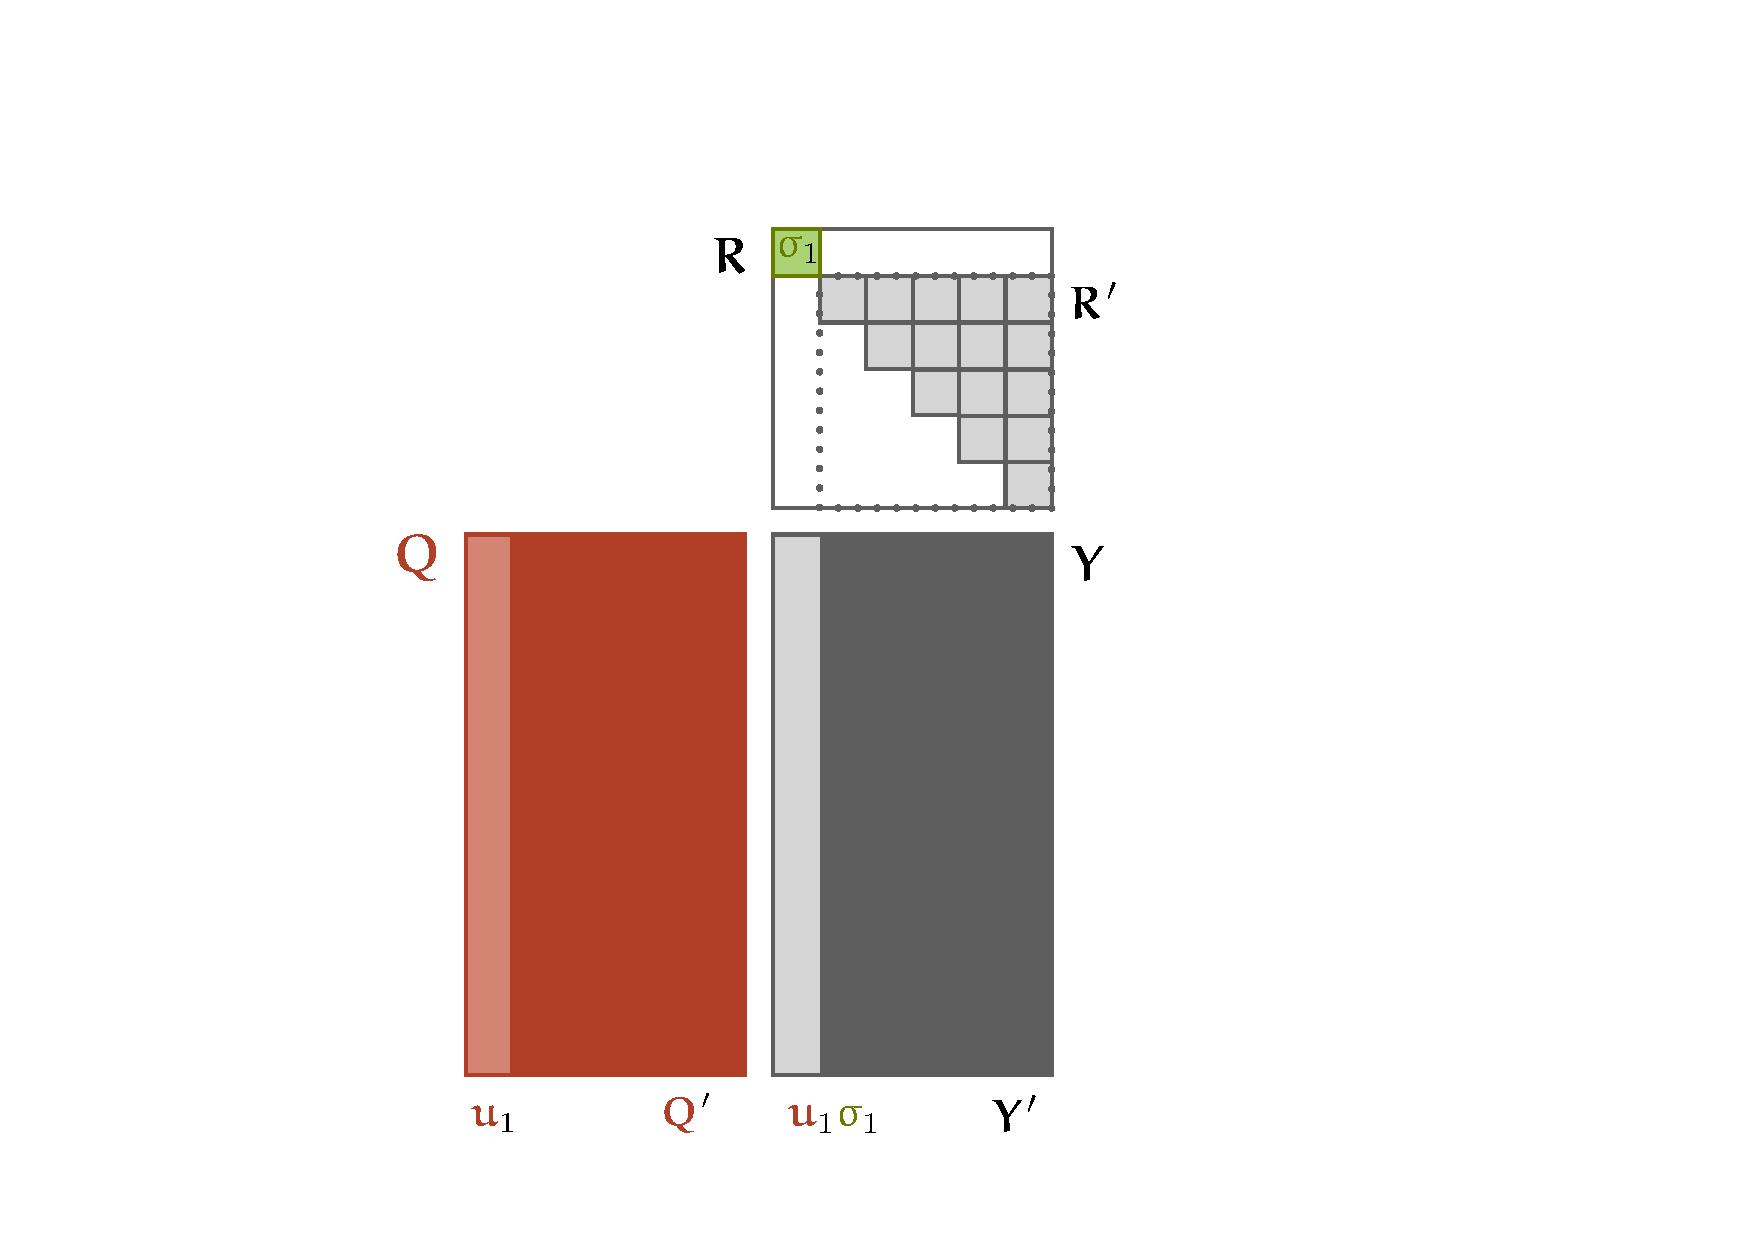
\includegraphics[width=0.5\textwidth]{./images/pca-5/subqr.pdf}
  }
  \caption*{The QR decomposition of the whole matrix \(\mbY\) contains the QR decomposition of the submatrix \(\mbY'\) (if its first column is a scalar multiple of \(\rc{\mbu}_1\)).}
\end{figure}

%<figure class="narrow centering">
%<img src="/images/pca-5/subqr.svg" class="half">
%<figcaption>The QR decomposition of the whole matrix \(\Y\) contains the QR decomposition of the submatrix \(\Y'\) (if its first column is a scalar multiple of \(\rc{\u}_1\)).
%</figcaption>
%</figure>

In the third line of the algorithm, we compute \(\mbY' \leftarrow \gc{\mbM}^T\rc{\mbQ}'\). Since \(\rc{\mbQ}'\) spans a subspace orthogonal to \(\rc{\mbu}_1\), by the same logic we used for line 1, \(\mbY'\) spans a subspace orthogonal to \(\rc{\mbv}_1\). 

Finally, we repeat the logic of line 2 to conclude that after the fourth line \(\rc{\mbP} = \left [\,\rc{\mbv}_1\;\rc{\mbp}'_1 \;\ldots\; \rc{\mbp}'_m\,\right]\). And that \(\mbB'\) is the bottom right submatrix of \(\mbB\).

To summarize, for a matrix \(\rc{\mbP}'\) with columns orthogonal to \(\rc{\mbv}_1\) and a matrix \(\rc{\mbP} = \left[\,\rc{\mbv}_1\;\rc{\mbp}'_1 \;\ldots\; \rc{\mbp}'_m\,\right]\), we have just shown that an iteration on \(\rc{\mbP}'\) produces matrices \(\rc{\mbQ}'\), \(\mbR'\), \(\rc{\mbP'}\) and \(\mbB'\), which are submatrices of the corresponding matrices we would get if we ran the iteration on \(\rc{\mbP}\).

This tells us directly that if \(\rc{\mbp}_2 = \rc{\mbv}_2\) before the iteration, by the argument we have already made above, this is a fixed point, and it will remain so after the iteration.

However, what if it isn't? It seems likely that the iteration with an arbitrary starting value for \(\rc{\mbp}_2\) will converge to \(\rc{\mbv}_2\) eventually. What we've shown above is, assuming \(\rc{\mbv}_1 = \rc{\mbp}_1\), that after the first iteration, where \(\rc{\mbp}_2\) is projected away from \(\rc{\mbv}_1\), it will remain orthogonal to \(\rc{\mbv}_1\) forever.

Since \(\rc{\mbp}_2\) is guaranteed to be orthogonal to \(\rc{\mbp}_1\) already, all that happens in the QR decomposition is that it is scaled to a unit vector. We can see this in the matrix \(\mbR\), where \(R_{12}\) is zero, and \(R_{22}\) (or \(R'_{11}\)) gives us the required scaling factor.

Under these assumptions, for \(\rc{\mbp}_2\) one iteration of the algorithm performs in order, a matrix multipliation, a scaling, a matrix multiplication and another scaling. Or, symbolically:

\[
\rc{\mbp}_2 \leftarrow L_{22}\gc{\mbM}^TR_{22}\gc{\mbM}\rc{\mbp}_2 = L_{22}R_{22}\gc{\mbM}^T\gc{\mbM}\rc{\mbp}_2  \p
\]

After \(k\) iterations, we get 

\[
\rc{\mbp}^k_2 = L_{22}\gc{\mbM}^TR_{22}\gc{\mbM}\rc{\mbp}_2 = (L_{22}R_{22})^k(\gc{\mbM}^T\gc{\mbM})^k\rc{\mbp}^0_2  \p
\]

This should look familiar. It shows that all we are doing is iteratively multiplying by \(\gc{\mbM}^T\gc{\mbM}\), and occasionally normalizing. Normally, such an iteration would converge to the \emph{first} eigenvector of \(\gc{\mbM}^T\gc{\mbM}\), and the first right singular vector of \(\gc{\mbM}\). However, by careful choice of the initial vector, we are constrained to be (and stay) orthogonal to that first eigenvector. As we've already seen in the orthogonal iteration for eigenvectors, this means that we will converge to the second eigenvector. 

Finally, we can repeat the same argument for the other vectors. If we set the first \emph{two} columns of \(\rc{\mbP}\) equal to \(\rc{\mbv}_1\) and \(\rc{\mbv}_2\) respectively, the same argument tells us that the algorithm will behave as though we are just iterating over the remaining columns, and will converge to the dominant singular vector in the remaining subspace. We can continue this process until all columns are exhausted.

In practice, of course, the second column doesn't need to wait until the first has converged. The closer \(\rc{\mbp}_1\) gets to \(\rc{\mbv}_1\), the better constrained the iteration on \(\rc{\mbp}_2\) will be to the correct subspace. By the time \(\rc{\mbp}_1\) has converged we are likely to see that \(\rc{\mbp}_2\) has also found its correct value. However, if it hasn't, we have just shown that it is guaranteed to once \(\rc{\mbp}_1 = \rc{\mbv}_1\).

\subsection{The QR algorithm for the SVD}

\index{QR algorithm!for SVD}
\index{Computing SVD!by the QR algorithm}

If only for the sake of symmetry, it would be nice if there were an SVD version of the QR iteration algorithm. Happily, it turns out there is, although we need to be careful to translate the logic of the QR iteration in the correct way. 

As before, we'll show the algorithm first, and then work out how it relates to the orthogonal iteration.
%
\begin{align*}
&\mbX, \mbY \leftarrow \gc{\mbM}, \gc{\mbM}^T \\
&\textbf{loop}\hspace{.2em}: \\
&\tab \rc{\mbQ}, \mbR \leftarrow \text{qr}(\mbX) \\
&\tab \rc{\mbP}, \mbB \leftarrow \text{qr}(\mbY) \\
&\tab \mbX \leftarrow \mbR\rc{\mbP}\\
&\tab \mbY \leftarrow \mbB\rc{\mbQ}
\end{align*}

Compared to the QR iteration for eigenvectors, things have become a little more complex. There, we just took a QR decomposition and multiplied it back in reverse order. Here, we take two QR decompositions, and we don't just multiply them back in reverse order, we also mix up the matrices, multiplying \(\mbR\) with \(\rc{\mbP}\) and \(\mbB\) with \(\rc{\mbQ}\).

\pagebreak\noindent As before, this algorithm only works if we compute the full QR decomposition. Here's what that looks like for a rectangular matrix.

\begin{figure}[H]
  \centerline{
	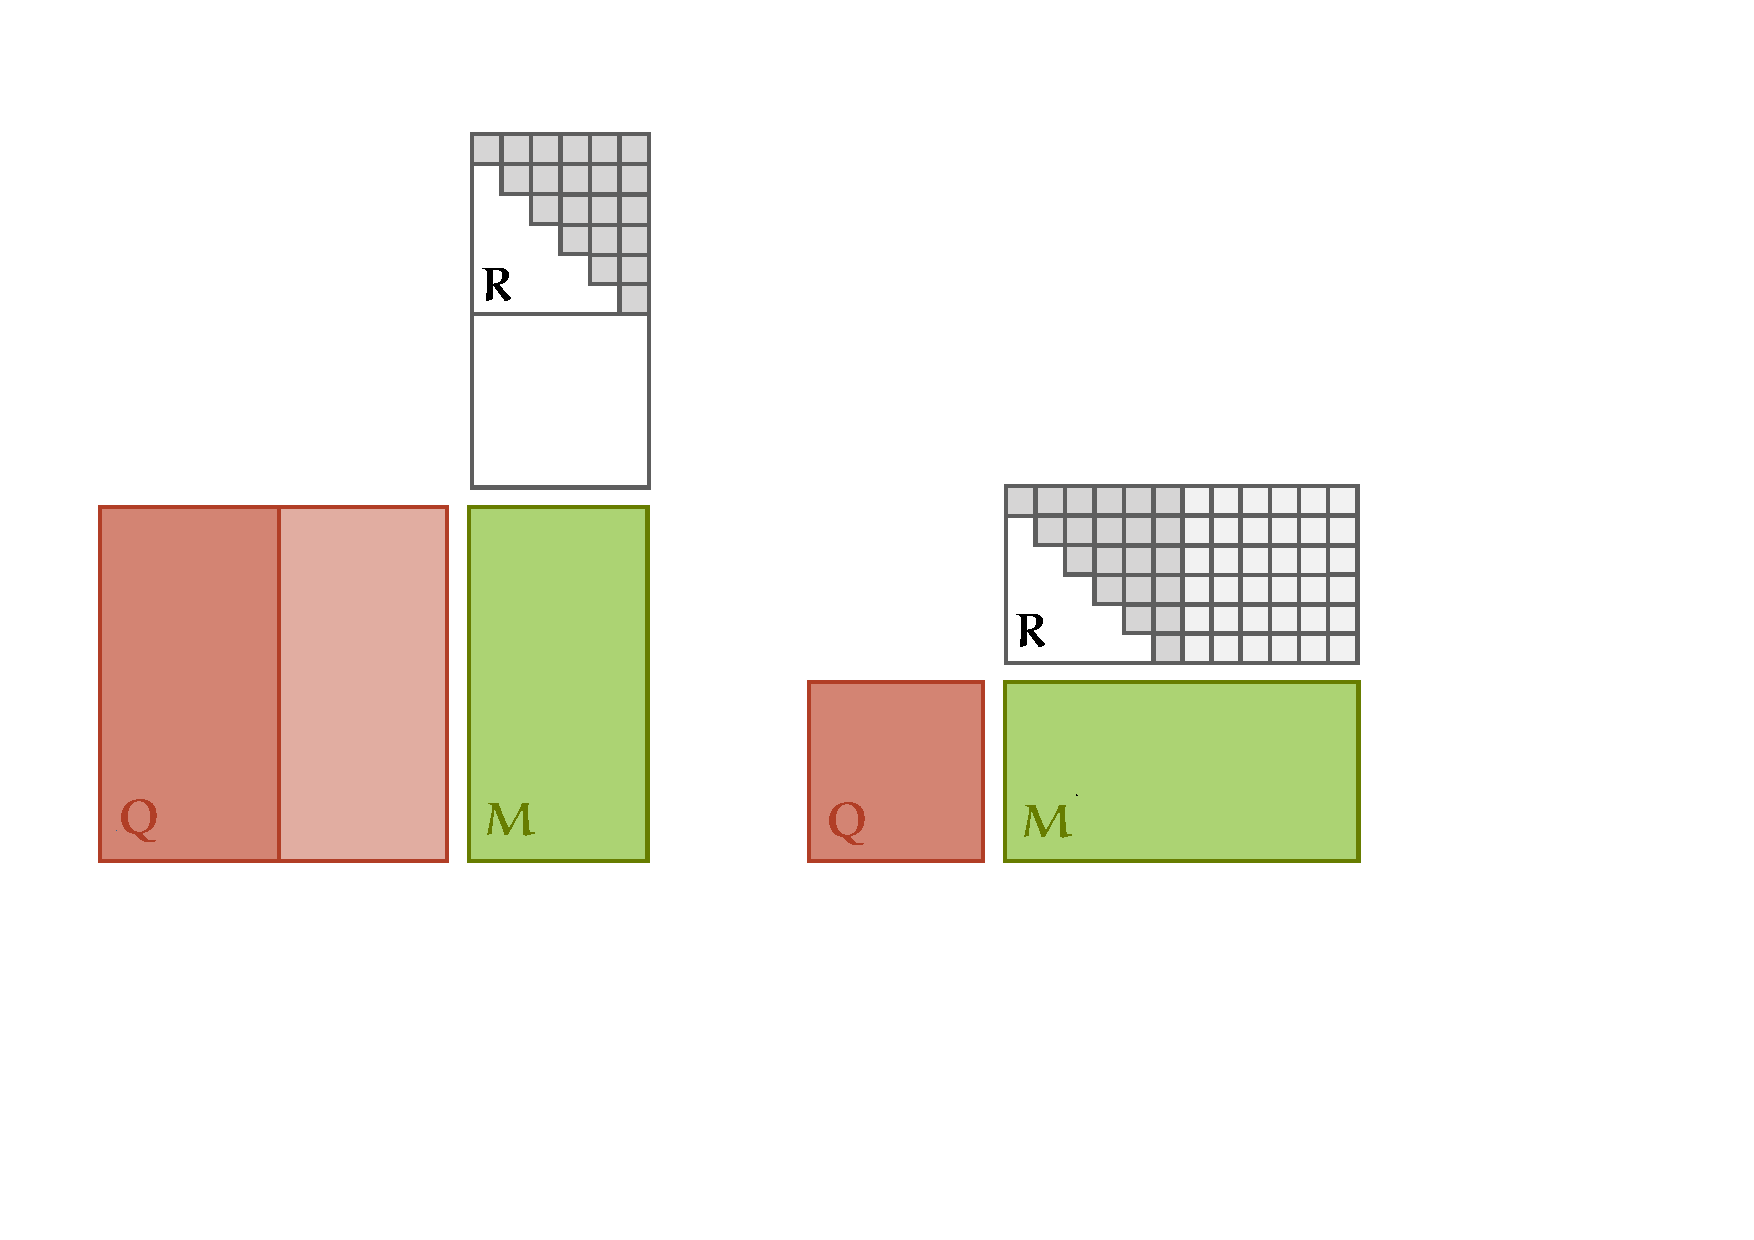
\includegraphics[width=1\textwidth]{./images/pca-5/rectangular-qr.pdf}
  }
\end{figure}

%<figure class="narrow centering">
%<img src="/images/pca-5/rectangular-qr.svg" >
%</figure>

\index{QR decomposition!for a rectangular matrix}

The key requirement is that \(\rc{\mbQ}\) is square. This means that if the matrix is tall, as it is on the left, we compute as many orthogonal vectors as the matrix has columns, and then extend this to a full basis by choosing arbitrary orthogonal vectors until \(\rc{\mbQ}\) is square. To make the multiplication work, we then extend \(\mbR\) with rows filled with zeros.

If the matrix is wide, the QR algorithm should provide us with a full basis. We now just need to extend \(\mbR\) far enough to make the multiplication of \(\rc{\mbQ}\) and \(\mbR\) reconstruct all columns of the matrix. Since we have a full basis with at least the dimensionality of the matrix, we know that the remaining columns are linear combinations of the columns of \(\rc{\mbQ}\). We express each remaining column of the matrix as a linear combination of the columns of \(\rc{\mbQ}\), giving us an additional column of \(\mbR\) until \(\mbR\) is as wide as \(\gc{\mbM}\).

Now, to work out why this is the algorithm that gives us the result we want, we'll need to carefully take the logic from the eigenvector version, and apply it here step-by-step. 

\pagebreak\noindent In the eigenvector version, two ideas were key:

\begin{enumerate}
\item We noted that the sequence of \(\mbR'\) matrices computed by the orthogonal algorithm was defined by \(\mbR'i = \rc{\mbQ}'_i\bc{\mbA}\rc{\mbQ}'_{i-1}\).\label{enum:step1}
\item We defined a sequence of new matrices \(\bc{\mbD}_i = {\rc{\mbQ}'_{i}}^T\bc{\mbA}\rc{\mbQ}'_i\), inspired by the equation that holds when the algorithm has converged.\label{enum:step2}
\end{enumerate}

We then showed that the sequence of \(\bc{\mbD}_i\)'s can be computed by taking the QR decomposition of the previous element, and multiplying it in reverse order, to produce the next.

Translating idea \ref{enum:step1} to the SVD version of the orthogonal iteration tells us that 

\begin{align*}
\rc{\mbQ}'_i\mbR'_i &= \gc{\mbM}\rc{\mbP}'_{i-1} &  \mbR'_i &= {\rc{\mbQ}'_i}^T\gc{\mbM}\rc{\mbP}'_{i-1} \\
\rc{\mbP}'_i\mbB'_i &= \gc{\mbM}^T\rc{\mbQ}'_{i} &  \mbB'_i &= {\rc{\mbP}'_i}^T\gc{\mbM}^T\rc{\mbQ}'_i \p 
\end{align*}

\begin{aside}On the left are simply the two QR decompositions computed in one iteration of the orthogonal algorithm. On the right, we've rewritten them to isolate \(\mbR'_i\) and \(\mbB'_i\)	
\end{aside}

To translate idea \ref{enum:step2} we note that at convergence, we can increment the index of the rightmost factor by one. That is, in the limit of \(i \to \infty\), the following equations hold:

\begin{align*}
\mbR'_i &= {\rc{\mbQ}'_i}^T\gc{\mbM}\rc{\mbP}'_{i} \\
\mbB'_i &= {\rc{\mbP}'_i}^T\gc{\mbM}^T\rc{\mbQ}'_{i+1}\p
\end{align*}

We now take these equations, and define new matrices \(\mbX_i\) and \(\mbY_i\) according to them. This is exactly the logic we used to define \(\bc{\mbD}_i\). In the limit they are equal to \(\mbR'_i\) and \(\mbB'_i\), but for small \(i\) there may be a large difference.

\begin{align*}
\mbX_i &= {\rc{\mbQ}'_i}^T\gc{\mbM}\rc{\mbP}'_{i} \\
\mbY_i &= {\rc{\mbP}'_i}^T\gc{\mbM}\rc{\mbQ}'_{i+1} \p 
\end{align*}

The final step is to show that in these sequences of \(\mbX_i\) and \(\mbY_i\) we can always compute the element at \(i\) by QR decomposing the elements at \(i-1\) and multiplying back in reverse order \emph{and mixing up the matrices}.

We'll start with elements \(\mbX_{i-1}\) and \(\mbY_{i-1}\). We'll need to express both of them as QR decompositions.

\begin{align*}
\mbX_{i-1} &= {\rc{\mbQ}'_{i-1}}^T \gc{\mbM} \rc{\mbP}'_{i-1} & \mbY_{i-1} &= {\rc{\mbP}'_{i-1}}^T  \gc{\mbM}^T \rc{\mbQ}'_{i} & \text{by definition} \\
\mbX_{i-1} &= {\rc{\mbQ}'_{i-1}}^T \rc{\mbQ}'_i \mbR'_i & \mbY_{i-1} &= {\rc{\mbP}'_{i-1}}^T \rc{\mbP}'_i\mbB'_i & \text{QR's in the orth. alg.} \\
\mbX_{i-1} &= \gc{{{\mbQ}'_{i-1}}^T {\mbQ}'_i} \mbR_i & \mbY_{i-1} &= \gc{{{\mbP}'_{i-1}}^T  {\mbP}'_i} \mbB'_i & \gc{\text{highlight}} \p \\
\end{align*}

In the last line, we haven't changed anything. We've only highlighted that we've ended up expressing both \(\mbX_{i-1}\) and \(\mbY_{i-1}\) as a QR decomposition. The \gc{two factors highlighted in green} are both orthogonal matrices, so their product is an orthogonal matrix as well, and the remainders \(\mbR_i\) and \(\mbB_i\) are upper triangular.

Now, we need to show that the next matrices in the sequence, \(\mbX_i\) and \(\mbY_i\), can be expressed in terms of the factors of these two QR decompositions. Starting with the definitions, we get

\begin{align*}
\mbX_i &= {\rc{\mbQ}'_i}^T\gc{\mbM}\rc{\mbP}'_i &  \mbB_i &= {\rc{\mbP}'_i}^T\gc{\mbM}^T\rc{\mbQ}'_{i+1} & \text{by definition} \\
&= {\rc{\mbQ}'_i}^T\gc{\mbM}{\rc{\mbP}'_{i-1}}^T\rc{\mbP}'_{i-1}\rc{\mbP}'_i & &= {\rc{\mbP}'_i}^T\gc{\mbM}^T{\rc{\mbQ}'_{i}}^T\rc{\mbQ}'_{i}\rc{\mbQ}'_{i+1} & \text{insert \(\mbI\)} \\
&= \kc{{{\mbQ}'_i}^T{\mbQ}'_i}\mbR'_i\rc{\mbP}'_{i-1}\rc{\mbP}'_i & &= \kc{{{\mbP}'_i}^T{\mbP}'_i}\mbB'_i\rc{\mbQ}'_{i}\rc{\mbQ}'_{i+1} & \text{from orth. alg.} \\
&= \mbR'_i\gc{{\mbP}'_{i-1}{\mbP}'_i} & &= \mbB_i\gc{{\mbQ}'_{i}{\mbQ}'_{i+1}} & \\
\end{align*}

<p>And there we have the proof that our algorithm converges to the right solution. If we QR decompose \(\mbX_{i-1}\) and \(\mbY_{i-1}\) and multiply the results back together, mixed up and in reverse order, we get the values \(\mbX_i\) and \(\mbY_i\). Since we know that these converge to the same values as the sequences \(\mbR'_i\) and \(\mbB'_i\), we see that we must be computing the singular value decomposition of \(\gc{\mbM}\).

\begin{aside}As before, the stripped down version we've given here only gives you the singular values (on the diagonal of \(\mbX\)). If you want the singular vectors as well, you'll need to keep a running product of \(\rc{\mbQ}\) and \(\rc{\mbP}\).
\end{aside}

This is where we will end our journey through the magical world of principal component analysis and all its relations. There is much we could still investigate. There are probabilistic and weighted versions of PCA. Regularized and sparse versions. There is a sidepath about non-linear PCA that could lead us into autoencoders, and from there into variational approaches in deep learning. Or, we could take a different track, and look into kernel-based nonlinear versions of PCA.

This is how it is, usually. The more you learn, the more the boundary of the unknown expands with it. It can be disheartening, especially if you're in the habit of focusing on all the things you don't yet know.

So let's allow ourselves a look back instead of forward, to see what we've accomplished. We may not know about all the ways in which PCA may be extended, and given more power by non-linear additions, but constrained to the purely linear domain, I think we can say we've covered the ground pretty thoroughly. 

We've seen the basic mechanism in operation, we've uncovered its connection to eigenvalues, we've proved the spectral theorem that the whole thing hinges on, and we've looked at the singular value decomposition, which provides a complementary perspective. Finally, in this last chapter, we've looked at a triad of algorithms for computing the eigendecomposition, and then adapted each in turn to provide us with the singular value decomposition instead.

Looking back, the aim of properly explaining PCA, down to its foundations has set us on a far more formidable journey than that initial challenge implied and, I must admit, than I originally anticipated. Taken together, these five chapters touch on almost all the topics that you might find in a standard linear algebra text book. From bases to (psuedo)inverses, to ranks and determinants. We may have entered the forest at a different point, and with a different goal, but our walk has covered much of the same ground. 

And that may be the best reason for an exercise like this. Let's be honest: you don't need to know all this to use PCA effectively. The first chapter of this book alone is more than enough to know what you are doing when you call the standard implementation in some data science library. However, true understanding of a concept comes from seeing it from different angles. So it is with the many building blocks of linear algebra. 

The explanations you find in a textbook will provide you, usually, with just one perspective. Enough for a basic grasp of the material, if you're lucky enough to remember what you learned. This kind of exercise, picking one method, and digging into it all the way down to the foundations, invariably requires you to revisit all those concepts you learned from the textbook, but with a new perspective, and a more concrete motivation.

If you're still reading at this point, that is hopefully what we've accomplished. To show how the whole cathedral of linear algebra works together to produce this magical operation that can take a messy, high-dimensional flood of data, and extract clean, low dimensional data, that more often than not, corresponds to the concepts we associate with its domain.

\vspace{5em}
\begin{figure}[H]
  \centerline{
	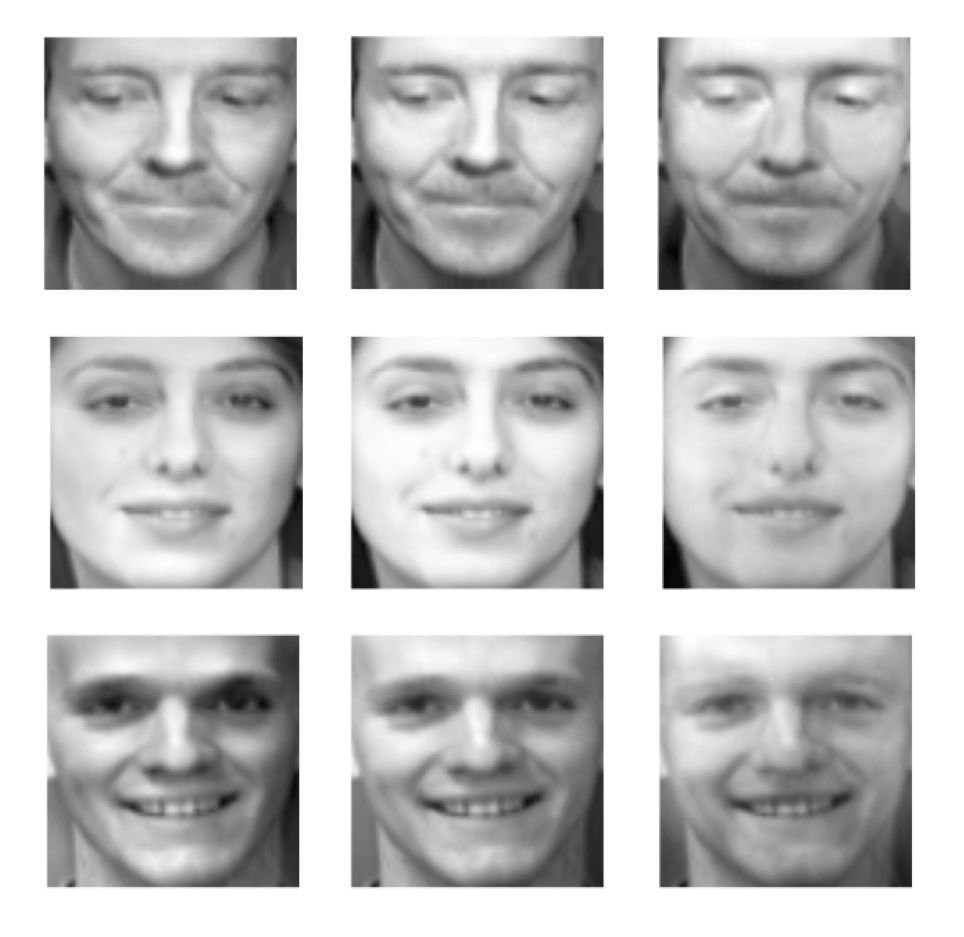
\includegraphics[width=0.5\textwidth]{./images/pca-5/faces.png}
  }
\end{figure}

%<figure class="narrow centering">
%<img src="/images/pca-5/faces.png" class="half"/>
%</figure>
